% =============================================================================
% Adaptive Check-In Workflows for Conversational Mental Health Companions:
% Scoping Review and Research Agenda
%
% Target venue: JMIR Mental Health (https://mental.jmir.org/)
% Article type: Review (Scoping Literature Review)
%
% Format: IMRD (Introduction / Methods / Results / Discussion) per JMIR's
%   Author Instructions for Reviews.
% Reporting standard: PRISMA-ScR (Tricco 2018) and PRISMA 2020 (Page 2021).
% Reference style: numeric (Vancouver / AMA-aligned), citation order,
%   typeset with biblatex+biber for source-side build reproducibility.
%   JMIR's typesetting team will reflow into the journal's house style at
%   acceptance; this file is the author-build representation.
% Build:  make    (uses latexmk + biber via the Makefile in this directory)
% =============================================================================

\documentclass[11pt,a4paper]{article}
\usepackage[T1]{fontenc}
\usepackage[utf8]{inputenc}
\usepackage[margin=1in]{geometry}
\usepackage{amsmath}
% Aggressive URL line-breaking. xurl supersedes url and lets URLs break
% at any character, which is essential for long footnote URLs and
% bibliographic DOIs that would otherwise cause Overfull \hbox warnings.
\PassOptionsToPackage{hyphens}{url}
\usepackage{xurl}
\usepackage{hyperref}
\usepackage{graphicx}
\usepackage{booktabs}
\usepackage{array}
\usepackage{tabularx}
\usepackage{xcolor}
\usepackage{microtype}
\usepackage{setspace}
\usepackage{titlesec}
\usepackage{tikz}
\usetikzlibrary{arrows.meta,positioning,shapes.geometric,shapes.misc,calc}

% --- Bibliography (biblatex + biber, numeric/Vancouver style for AMA-alignment)
% JMIR uses AMA Manual of Style 11th edition: numbered references in citation
% order. biblatex 'numeric-comp' with sorting=none provides the closest
% author-build equivalent; JMIR typesetting will normalise to AMA at
% acceptance.
\usepackage[
  backend=biber,
  style=numeric-comp,
  sorting=none,
  doi=true,
  url=false,
  isbn=false,
  giveninits=true,
  uniquename=init,
  maxbibnames=8,
  minbibnames=6
]{biblatex}
\addbibresource{references.bib}

% Suppress internal Scite-verification provenance notes from the printed
% bibliography. Notes remain in source as an audit trail.
\AtEveryBibitem{\clearfield{note}}

% Add a tiny stretch to inter-character glue inside URLs so xurl can
% break them without leaving overfull boxes. xurl already breaks at any
% character; this just gives TeX a little more flexibility when justifying.
\Urlmuskip=0mu plus 1mu

% --- Title and front matter ---------------------------------------------------
\title{Adaptive Check-In Workflows for Conversational
Mental Health Companions:\\Scoping Review and Research Agenda}

\author{Majid Memari, PhD\\
Department of Computer Science\\
Utah Valley University, Orem, UT, USA\\
ORCID: 0000-0001-5654-4996\quad
\texttt{mmemari@uvu.edu}}
\date{}

\hypersetup{
  pdftitle={Adaptive Check-In Workflows for Conversational Mental Health Companions: Scoping Review and Research Agenda},
  pdfauthor={Majid Memari},
  pdfkeywords={mHealth; mental health; conversational agent; chatbot;
    large language model; just-in-time adaptive intervention;
    micro-randomized trial; scoping review; digital therapeutic alliance;
    behavior change; agentic workflow},
  hidelinks
}

\sloppy

% Cross-referencing macros.
\newcommand{\secref}[1]{Section~\ref{#1}}
\newcommand{\tabref}[1]{Table~\ref{#1}}
\newcommand{\figref}[1]{Figure~\ref{#1}}

% Tighten the spacing on standard \paragraph (sectioning level 4) so the
% inline bold lead-ins look like dense scientific writing rather than
% loose headings. We keep \paragraph as a real sectioning command so that
% hyperref's PDF bookmarks and microtype's footnote patches both work.
\titlespacing*{\paragraph}{0pt}{0.5\baselineskip}{0.5em}

\begin{document}

\maketitle

\begin{flushleft}
\textbf{Article type:} Review (Scoping Literature Review)
\end{flushleft}

% =============================================================================
% Structured Abstract -- JMIR Mental Health requires a structured abstract
% with the headers Background / Objective / Methods / Results / Conclusions,
% maximum 450 words, with adherence to PRISMA for Abstracts recommended.
% =============================================================================
\section*{Abstract}

\paragraph{Background.}
Conversational artificial intelligence (AI) for mental health has
matured rapidly. Randomized controlled trials of cognitive behavioral
chatbots have produced clinically measurable symptom reductions;
generative-AI chatbots have produced large-effect improvements on
clinical outcomes (Cohen $d\!=\!0.79\text{--}0.90$); and
meta-analyses of app-supported smartphone interventions for mental
health show small-to-moderate effects (Hedges $g\!\approx\!0.28\text{--}0.58$).
Despite this progress, no peer-reviewed deployment combines a
\emph{learned, longitudinal model of the client}, a \emph{theory-grounded
scheduling policy} that selects when to reach out and what to offer, a
\emph{multi-framework intervention library} authored by the subject
matter expert (SME) and selected from by the policy, and a
\emph{crisis-safe conversational substrate}---all evaluated on
listener-centered outcomes.

\paragraph{Objective.}
This scoping review synthesizes the literatures of just-in-time
adaptive interventions (JITAIs), micro-randomized trials (MRTs),
conversational mental health agents, and the digital therapeutic
alliance (DTA) to assess whether an integrated, adaptive check-in
workflow can be assembled today using existing methods, and to
specify a research agenda for evaluating one.

\paragraph{Methods.}
We followed the Arksey--O'Malley five-stage framework with the
methodological refinements of Levac et al., and report findings
according to the PRISMA Extension for Scoping Reviews (PRISMA-ScR).
Twelve Boolean queries spanning three thematic pillars
(\emph{Sense}, \emph{Decide}, \emph{Act}) and six cross-cutting concerns
(therapeutic frameworks, wellbeing techniques, crisis safety,
engagement, ethics, evaluation methodology) were executed in
April~2026 against PubMed/MEDLINE, PsycINFO (via Ovid), and Scopus,
with citation-context verification through the Scite verified-DOI
service for every source retained for synthesis. We applied
prespecified inclusion criteria (verified DOI; peer-reviewed venue
or recent foundational preprint with $\ge\!5$ citing publications;
topical relevance to one of eight research questions; sufficient
methodological detail) and synthesized findings narratively across
the three pillars and six cross-cutting concerns.

\paragraph{Results.}
We synthesized 62 verified-DOI sources. The \emph{Sense} pillar
offers a mature methodological chain from ecological momentary
assessment through passive sensing and digital phenotyping to
large-language-model (LLM) state inference. The \emph{Decide} pillar
provides the most developed methodological stack: a JITAI conceptual
framework, MRT evaluation design with statistical machinery,
contextual-bandit and reinforcement-learning policy classes with
both online and offline precedent, and one mental-health-relevant
adaptive-messaging RCT (DIAMANTE). The \emph{Act} pillar contributes
RCT-validated chatbot precedents (Woebot, Wysa, Therabot), recent
meta-analytic effects on the order of $g\!\approx\!0.28\text{--}0.64$
across depressive and anxious symptoms, an attrition baseline of
$\sim\!22\%$ for chatbot RCTs, and an evolving DTA literature.
Cross-cutting findings cover therapeutic-framework evidence bases,
wellbeing-technique mechanisms, crisis-safety architectures,
engagement and attrition baselines, ethical constraints, and
evaluation instruments. We define five operational integration
criteria (C1--C5) and find no peer-reviewed system that demonstrably
satisfies all five jointly. A subsystem-by-subsystem feasibility
analysis indicates that every component required to fill the gap
appears available from existing methods, instruments, and currently
available models.

\paragraph{Conclusions.}
The integration of a learned, theory-grounded, scheduled check-in
workflow into a multi-framework conversational mental health
companion appears methodologically tractable today but has not been
attempted in peer-reviewed deployment. We propose a
\emph{Decide-first} prototype evaluated by an MRT against a
fixed-cadence baseline, with proximal-effect, alliance, and
retention reporting. The literature supports the design; the
prototype, the trial, and the clinical or behavioral outcomes are
explicitly future work.

\paragraph{Keywords.}
mHealth; mental health; conversational agent; chatbot; large language
model; just-in-time adaptive intervention; micro-randomized trial;
scoping review; digital therapeutic alliance; behavior change.

% =============================================================================
\section{Introduction}\label{sec:introduction}

\subsection{Background}\label{sec:bg}

Conversational artificial intelligence (AI) for mental health has
made rapid empirical progress. The Woebot RCT of Fitzpatrick et
al.~\cite{Fitzpatrick2017Woebot}, the Wysa real-world evaluation of
Inkster et al.~\cite{Inkster2018Wysa}, and the
\textit{NEJM~AI} Therabot RCT of Heinz et
al.~\cite{Heinz2025TherabotRCT} collectively demonstrate that
chat-substrate interventions can produce clinically meaningful
symptom reductions and therapist-comparable alliance ratings. The
meta-analytic baseline across 66 smartphone-intervention RCTs in the
Linardon et al.\ synthesis~\cite{Linardon2019Meta} is
$g\!\approx\!0.28\text{--}0.58$ across depression, anxiety, stress,
quality-of-life, and social-anxiety outcomes, with cognitive
behavioral therapy (CBT)-based apps with engagement support producing
the largest effects. This empirical base is sufficient to justify
continued deployment of supportive conversational companions; it is
\emph{not} sufficient to claim the field has found the right shape
for them.

\subsection{Prior Work and Persistent Gaps}\label{sec:prior-work}

Three deeper gaps persist across the published corpus.
(a)~\emph{No longitudinal learned model of the client.} Most chatbot
deployments rely on static intake forms or implicit context windows;
they do not learn what this user is like over weeks or months in
ways that can transfer across sessions.
(b)~\emph{No theory-grounded scheduling policy.} Delivery schedules
are typically fixed (daily check-in, weekly session) or entirely
user-initiated; the extensive literature on just-in-time adaptive
interventions (JITAIs), micro-randomized trials (MRTs), and
contextual-bandit / reinforcement-learning (RL) policies developed
in mobile-health
biostatistics~\cite{NahumShani2018JITAI,Klasnja2015MRT,Liao2020PersonalizedHeartSteps}
has been applied to physical-activity outcomes and, in one recent
study~\cite{Aguilera2024DIAMANTERL}, to depression-relevant
populations via text messaging, but has not been integrated into a
multi-framework conversational mental health companion.
(c)~\emph{No multi-framework intervention library bound to a
scheduling policy.} Most chatbots commit to a single therapeutic
framework at design time; the subject matter expert (SME) who knows
the audience has no seam through which to swap in acceptance and
commitment therapy (ACT), motivational interviewing (MI), dialectical
behavior therapy (DBT) skills, or compassion-focused therapy (CFT),
and no scheduling intelligence that learns which move to select for
which state.

\subsection{Objective and Research Questions}\label{sec:objective}

The objective of this scoping review is twofold: (1) to synthesize
the literatures that bear on those three gaps and (2) to ask whether
they can be filled with currently available methods. We organize the
field around three pillars and six cross-cutting concerns:

\begin{itemize}\setlength{\itemsep}{0pt}
  \item \emph{Sense} (Section~\ref{sec:sense}): how can a system
    build a longitudinal, psychologically meaningful model of a
    client from the conversation itself (and, optionally, light-touch
    ecological momentary assessment, EMA)?
  \item \emph{Decide} (Section~\ref{sec:decide}): when and what
    should the system deliver---how does the field connect
    JITAI/MRT/contextual-bandit policy mathematics to conversational
    mental health content?
  \item \emph{Act} (Section~\ref{sec:act}): how are chat-delivered
    interventions performing empirically, and what does the digital
    therapeutic alliance (DTA) literature say about the mediator
    between delivery and outcomes?
  \item Cross-cutting concerns: therapeutic
    frameworks~(Section~\ref{sec:frameworks});
    wellbeing techniques~(Section~\ref{sec:techniques}); crisis
    detection and safety~(Section~\ref{sec:safety});
    engagement and attrition~(Section~\ref{sec:engagement}); ethics,
    regulation, equity, and privacy~(Section~\ref{sec:ethics-results});
    and evaluation methodology~(Section~\ref{sec:evaluation}).
\end{itemize}

A future implementation need not be limited to language alone:
opt-in wearable signals (sleep, activity, heart-rate variability,
temperature, recovery
proxies)~\cite{Sequeira2021PassiveSensing,Laborde2017HRV} can
provide a lightweight sensing branch into the \emph{Sense} layer
that helps the \emph{Decide} policy time low-risk interventions
(grounding, paced breathing, reflective check-ins) at moments of
heightened stress, fatigue, or dysregulation, without establishing
a diagnosis on their own.

The review answers eight research questions, summarized in
\tabref{tab:rqs}. The synthesis is illustrated throughout against
one candidate architecture (named in Section~\ref{sec:conclusions})
that exemplifies each design commitment in concrete form; that
architecture is presented as an exemplar, not as the unit of
evaluation.

\paragraph{Scope of the present paper.}
This is a scoping literature review and research agenda, not a
system or evaluation paper. The candidate architecture referenced
in the Discussion currently realizes only the conversational
delivery layer with a baseline keyword crisis stack; the
\emph{Sense} layer, the \emph{Decide} scheduling policy, the
micro-randomized trial, and any clinical or behavioral outcomes
that this review motivates are explicitly positioned as future work
(Section~\ref{sec:conclusions}). No human subjects have been
recruited and no proximal or distal outcomes are reported in the
present paper.

\begin{table}[t]
\small
\begin{tabularx}{\textwidth}{l X}
\toprule
\textbf{ID} & \textbf{Research question} \\
\midrule
RQ1 & How can a longitudinal psychological model of the client be built from conversational data alone? \\
RQ2 & What JITAI / contextual-bandit / RL methodology is available, and what has it already produced in mental-health-adjacent trials? \\
RQ3 & What proximal and distal effect sizes should a chat-based mental health intervention plan to detect? \\
RQ4 & What digital therapeutic alliance instrument(s) should a prototype-scale evaluation use? \\
RQ5 & Which therapeutic frameworks have sufficient meta-analytic support for the SME to select as a primary method? \\
RQ6 & What is the evidence base for the wellbeing techniques (paced breathing, sensory grounding, cognitive reframing, self-compassion break) most commonly shipped as actions in supportive companions? \\
RQ7 & How should crisis detection be layered on top of, or alongside, an LLM chat substrate? \\
RQ8 & What engagement / adherence baseline should an adaptive scheduling policy be benchmarked against? \\
\bottomrule
\end{tabularx}
\caption{Research questions guiding this scoping review.}
\label{tab:rqs}
\end{table}

% =============================================================================
\section{Methods}\label{sec:methods}

\subsection{Study Design and Reporting Standards}\label{sec:design}

This is a scoping review that adopts the Arksey--O'Malley five-stage
framework~\cite{Arksey2005Scoping} with the methodological
refinements of Levac et al.~\cite{Levac2010Scoping}, and follows the
PRISMA Extension for Scoping Reviews (PRISMA-ScR)~\cite{Tricco2018PRISMAScR}
for reporting. We additionally align with PRISMA~2020~\cite{Page2021PRISMA}
where applicable. The completed PRISMA-ScR checklist is provided in
Multimedia Appendix 1. This is not a fully systematic review in the
clinical-trials sense; the heterogeneity of evaluation designs across
human--computer interaction (HCI), mobile-health biostatistics,
clinical psychology, and natural language processing does not support
a single quantitative pooling.

\subsection{Eligibility Criteria}\label{sec:eligibility}

\paragraph{Inclusion criteria.}
(i)~Verified DOI; (ii) peer-reviewed venue, or a recent foundational
preprint (e.g., arXiv) with $\ge\!5$ citing publications; (iii)
topical relevance to one of the eight research questions
(\tabref{tab:rqs}); (iv) sufficient methodological detail to
support the claim being cited.

\paragraph{Exclusion criteria.}
Retracted publications or papers flagged with editorial concerns
(checked via Scite \texttt{retraction\_notices} and
\texttt{has\_retraction} / \texttt{has\_concern} filters);
non-English publications without published translation; duplicates
of arXiv preprints already cited via their archival venue.

\subsection{Information Sources}\label{sec:sources}

Three peer-reviewed bibliographic databases were searched: PubMed /
MEDLINE (\url{https://pubmed.ncbi.nlm.nih.gov}), PsycINFO via Ovid,
and Scopus (\url{https://www.scopus.com}). Every record retained for
synthesis was additionally cross-checked against the Scite
verified-DOI service (\url{https://api.scite.ai}) to obtain
smart-citation context (supporting / contrasting / mentioning /
unclassified) and editorial-notice flags (retractions, concerns,
errata, corrections); papers flagged as retracted or with active
concern were excluded at full-text screening. Citation snowballing
was performed forward and backward from key reviews and RCTs
(notably Vaidyam et al.~\cite{Vaidyam2019ChatbotsReview,Vaidyam2021ChatbotLandscape},
He et al.~\cite{He2023CASRMeta}, Li et al.~\cite{Li2023AICAMeta},
Jabir et al.~\cite{Jabir2024AttritionMeta}, Guo et
al.~\cite{Guo2024LLMMHReview}, and Hua et
al.~\cite{Hua2025LLMScopingReview}) to surface sources that were
indexed in adjacent corpora (e.g., behavior-change taxonomy or
psychophysiology) but not retrieved by the primary database queries.
Industry and press sources were retrieved separately and are
treated as dated snapshots, never as load-bearing scientific
evidence. Searches were executed in April~2026 with no end-date
filter and a soft start date of~2014 (the year of the first formal
JITAI position paper) unless an earlier foundational reference was
needed (e.g., Arksey and O'Malley's 2005
framework~\cite{Arksey2005Scoping}; Hatcher and Gillaspy's 2006
WAI-SR validation~\cite{Hatcher2006WAISR}; Hofmann et al.'s 2012
CBT meta-analytic synthesis~\cite{Hofmann2012CBTMeta}).

\subsection{Search Strategy}\label{sec:search}

Searches were structured around twelve Boolean queries spanning the
three pillars and six cross-cutting concerns of the synthesis. Each
query was executed in PubMed/MEDLINE, PsycINFO (Ovid), and Scopus
with database-appropriate field tags; the abbreviated search terms
appear below, and the full per-database query strings, filters,
record counts, and post-screening retention are provided in
Multimedia Appendix~2.

\begin{itemize}\setlength{\itemsep}{0pt}
  \item Q1 (\emph{Decide}): \texttt{"just-in-time adaptive intervention" AND mental}
  \item Q2 (\emph{Decide}): \texttt{"micro-randomized trial" AND (mhealth OR "digital health")}
  \item Q3 (\emph{Decide}): \texttt{"contextual bandit" AND ("digital health" OR mhealth OR "behaviour change")}
  \item Q4 (\emph{Act}): \texttt{("chatbot" OR "conversational agent") AND ("depression" OR "anxiety" OR "mental health") AND (RCT OR trial)}
  \item Q5 (\emph{Act}): \texttt{"large language model" AND ("mental health" OR "psychotherapy" OR "counselling")}
  \item Q6 (\emph{Act}): \texttt{"therapeutic alliance" AND (chatbot OR "conversational agent" OR AI)}
  \item Q7 (\emph{Sense}): \texttt{"ecological momentary assessment" AND (depression OR anxiety OR affect)}
  \item Q8 (\emph{Frameworks}): \texttt{"behaviour change wheel" OR "behaviour change technique" AND digital}
  \item Q9 (\emph{Frameworks}): \texttt{("acceptance and commitment therapy" OR "motivational interviewing" OR "cognitive behavioural therapy") AND (digital OR app OR chatbot)}
  \item Q10 (\emph{Techniques}): \texttt{"slow breathing" AND ("heart rate variability" OR vagal)}
  \item Q11 (\emph{Techniques}): \texttt{"self-compassion" AND (intervention OR trial)}
  \item Q12 (\emph{Safety}): \texttt{"Columbia Protocol" OR "Columbia Suicide Severity Rating Scale" OR "Zero Suicide"}
\end{itemize}

\subsection{Selection of Sources of Evidence}\label{sec:selection}

The twelve queries returned 4{,}864 records across PubMed/MEDLINE
($n\!=\!4{,}854$ as the union of the per-query counts in Multimedia
Appendix~2), PsycINFO, and Scopus, plus 47 records identified
through citation snowballing from the six anchor reviews
in~\secref{sec:sources}. After de-duplication across databases
($n\!=\!927$ duplicates removed), 3{,}984 unique records were
screened at title and abstract by the single author against the
inclusion criteria of \secref{sec:eligibility}. Title and abstract
screening excluded 3{,}681 records (3{,}214 outside scope of the
eight research questions; 401 not peer-reviewed and not preprints
meeting the $\ge\!5$ citing publications threshold; 66 non-English
without published translation). Full text was sought for 303
records and obtained for 298 (5 not retrievable). Full-text
screening excluded a further 236 records (147 insufficient
methodological detail; 58 off-topic on full read; 22 preprint
duplicates of an archival venue already cited; 7 retracted or with
active editorial concern via Scite; 2 duplicates across databases
not caught at deduplication). Sixty-two records were retained for
synthesis. The flow is shown in \figref{fig:prisma}.

\begin{figure}[tbp]
\centering
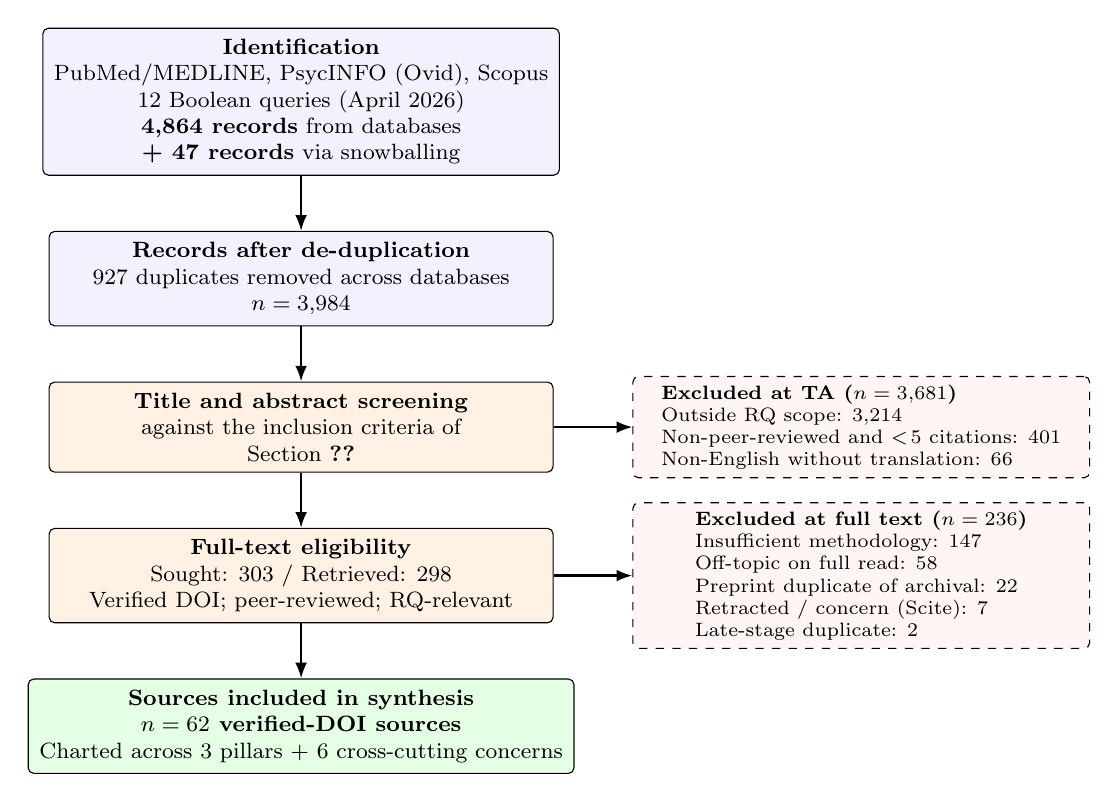
\begin{tikzpicture}[
  node distance=7mm and 10mm,
  every node/.style={font=\footnotesize},
  block/.style={rectangle, draw, rounded corners=2pt, align=center,
                inner sep=4pt, minimum width=64mm},
  side/.style={rectangle, draw, dashed, rounded corners=2pt, align=left,
                inner sep=3pt, font=\scriptsize, fill=red!4,
                minimum width=58mm},
  arr/.style={-{Latex[length=2mm]}, thick},
]
\node[block, fill=blue!5]   (id)    {\textbf{Identification}\\
                                     PubMed/MEDLINE, PsycINFO (Ovid), Scopus\\
                                     12 Boolean queries (April 2026)\\
                                     \textbf{4{,}864 records} from databases\\
                                     \textbf{+ 47 records} via snowballing};
\node[block, below=of id, fill=blue!5]
                            (dedup) {\textbf{Records after de-duplication}\\
                                     927 duplicates removed across databases\\
                                     \textbf{$n=3{,}984$}};
\node[block, below=of dedup, fill=orange!10]
                            (screen){\textbf{Title and abstract screening}\\
                                     against the inclusion criteria of\\
                                     Section~\ref{sec:eligibility}};
\node[side, right=of screen]
                            (excl1) {\textbf{Excluded at TA ($n=3{,}681$)}\\
                                     Outside RQ scope: 3{,}214\\
                                     Non-peer-reviewed and $<\!5$ citations: 401\\
                                     Non-English without translation: 66};
\node[block, below=of screen, fill=orange!10]
                            (full)  {\textbf{Full-text eligibility}\\
                                     Sought: 303 / Retrieved: 298\\
                                     Verified DOI; peer-reviewed; RQ-relevant};
\node[side, right=of full]
                            (excl2) {\textbf{Excluded at full text ($n=236$)}\\
                                     Insufficient methodology: 147\\
                                     Off-topic on full read: 58\\
                                     Preprint duplicate of archival: 22\\
                                     Retracted / concern (Scite): 7\\
                                     Late-stage duplicate: 2};
\node[block, below=of full, fill=green!10]
                            (incl)  {\textbf{Sources included in synthesis}\\
                                     \textbf{$n=62$ verified-DOI sources}\\
                                     Charted across 3 pillars + 6 cross-cutting concerns};

\draw[arr] (id) -- (dedup);
\draw[arr] (dedup) -- (screen);
\draw[arr] (screen) -- (full);
\draw[arr] (full) -- (incl);
\draw[arr] (screen) -- (excl1);
\draw[arr] (full) -- (excl2);
\end{tikzpicture}
\caption{PRISMA-ScR-style flow of records through identification,
screening, eligibility, and inclusion across PubMed/MEDLINE,
PsycINFO, and Scopus, with citation-context verification through
Scite at full-text screening.}
\label{fig:prisma}
\end{figure}

\subsection{Data Charting Process}\label{sec:charting}

For each retained source we extracted: bibliographic metadata
(authors, year, venue, DOI), Scite editorial-notice status, study
design, population, intervention or model under study, primary
outcome and effect-size estimate where available, and the pillar /
cross-cutting concern under which the source is cited in this
review. Charting was performed by the single author
(see~\secref{sec:limitations}).

\subsection{Synthesis of Results}\label{sec:synthesis-method}

We synthesized findings narratively, following the PRISMA-ScR
recommendation that scoping reviews map a body of literature rather
than pool effect sizes~\cite{Tricco2018PRISMAScR}. The synthesis
structure follows the Sense $\to$ Decide $\to$ Act loop described in
\secref{sec:objective}: \emph{Sense} maps the literature on learning
the client over time; \emph{Decide} maps the literature on adaptive
scheduling policies; \emph{Act} maps the literature on chat-substrate
intervention delivery. Six cross-cutting concerns frame the
remaining sections. Where directly comparable, we report effect-size
estimates in the original units (Cohen $d$, Hedges $g$, percentage
gain).

\subsection{Ethical Considerations}\label{sec:ethics-methods}

This is a literature review and contains no new human-subjects data;
Institutional Review Board (IRB) approval was not required and no
participants were recruited. The review nonetheless touches several
ethics-relevant areas (mental-state inference as surveillance risk;
engagement-optimization as misaligned reward; crisis-handoff
responsibility; scope and equity), addressed in
\secref{sec:ethics-results} and revisited in
\secref{sec:limitations}.

% =============================================================================
\section{Results}\label{sec:results}

\subsection{Selection and Characteristics of Sources of Evidence}\label{sec:char}

The synthesis draws on 62 verified-DOI sources retained from the
selection process described in \secref{sec:selection} and
\figref{fig:prisma}. \tabref{tab:taxonomy} summarizes the design
space these sources cover. The bibliography mirrors this structure
with twelve labeled sections (0~Methodology; A~Sense; B~Decide;
C~Act; C+~additional chatbot/LLM reviews and meta-analyses;
D~Therapeutic frameworks; E~Wellbeing techniques; F~Crisis
detection and safety; G~Engagement and attrition; H~Ethics,
regulation, equity, privacy; I~Evaluation methodology; J~Industry
/ press snapshots).

\begin{table}[t]
\small
\begin{tabularx}{\textwidth}{l X}
\toprule
\textbf{Axis} & \textbf{Design positions covered by this review} \\
\midrule
Client model (Sense) & Static intake (most chatbots); EMA-augmented; passive-sensing-augmented; wearable-augmented (watch/ring); LLM-state-inference from chat. Scoped here primarily to the last two. \\
Input modality & Chat-only (baseline), chat $+$ EMA, chat $+$ passive sensing, chat $+$ wearable (e.g., watch/ring signals such as sleep, activity, HRV, temperature). A pragmatic first implementation would typically start chat-only. \\
Policy class (Decide) & Fixed cadence; rule-based decision tree; contextual bandit; RL. We adopt CMAB / RL as the target policy class with MRT evaluation. \\
Action menu (Decide $+$ Act) & Single-framework catalogue (Woebot, Wysa); multi-framework SME-authored catalogue; BCT-taxonomy-aligned. \\
Delivery substrate (Act) & Rule-based chat, fine-tuned generative-AI chat, general LLM $+$ prompt-engineered content. \\
Crisis layer & Keyword-only; keyword $+$ moderation API; keyword $+$ LLM safety classifier; C-SSRS-validated. A pragmatic first implementation may begin keyword-only. \\
Therapeutic framework & CBT; ACT; MI; DBT skills; person-centered; CFT; SFBT. SME-selectable. \\
Engagement strategy & None; reminders; gamification; adaptive schedule (the claim of this review). \\
Evaluation surface & Symptom scales (PHQ-9, GAD-7); WAI-SR digital therapeutic alliance; MRT proximal effects; retention curves. \\
Governance surface & Consent and disclosure; content-author separation; no-persistence default; documented governance architecture. \\
\bottomrule
\end{tabularx}
\caption{Design space for conversational mental health companions
synthesized by this review.}
\label{tab:taxonomy}
\end{table}

\subsection{Pillar A: Sense---Learning the Client Over Time}\label{sec:sense}

The Sense pillar asks: \emph{how can a system build a reliable,
longitudinal, psychologically meaningful model of an individual
client without crossing into surveillance, and using only the
channels actually available to a conversational mental health
companion?} For a chat-based companion this means, primarily,
\emph{the conversation itself}, and (optionally, in future
deployments) light-touch EMA prompts and, where a user explicitly
opts in, lightweight wearable-derived state signals from devices
such as watches and rings. Heavy passive sensing is held out of
scope by design, since SME-authored boundaries in a companion's
content layer typically forbid persistent capture without consent,
and the legal and sociological cost of that data class is high
(\secref{sec:ethics-results}). The literature reviewed here
therefore divides into four threads, ordered from most to least
directly applicable to a chat-only baseline.

\paragraph{Ecological momentary assessment as the conceptual anchor.}
EMA was formalized by Stone and Shiffman in 1994 and matured into a
mainstream clinical-assessment method through the 2000s; the most
useful synthesis for a digital-mental-health implementer is
Trull and Ebner-Priemer~\cite{Trull2009ESMEMA}, the special-section
introduction in \emph{Psychological Assessment} that defines EMA as
in-the-moment, real-world, repeated sampling of states and
behaviors. EMA's two empirical commitments---ecological validity
and the avoidance of retrospective recall bias---transfer directly
to a chat-based check-in workflow. Versluis et
al.~\cite{Versluis2016EMI} extend the EMA paradigm into
\emph{ecological momentary interventions} (EMIs) for depression and
anxiety: brief, in-context interventions delivered in response to a
detected state. EMI is the conceptual ancestor of the JITAI
literature in Pillar~B; together they motivate the
Sense$\,\to\,$Decide handoff this synthesis foregrounds.

\paragraph{Passive sensing as the upper bound.}
Two reviews delineate the modern landscape of passive sensing for
mental health monitoring. Cornet and Holden~\cite{Cornet2018PassiveSensing}
systematize the smartphone-only literature and find that step
counts, location clusters, screen time, and inter-event timing
yield modest but reproducible signal on depressive symptoms;
reliability is bounded by sensor noise, user-context drift, and
missing-data patterns that correlate with the clinical state being
measured. Sequeira et al.~\cite{Sequeira2021PassiveSensing} broaden
the picture to wearable and environmental sensors and confirm that
multimodal passive sensing outperforms any single modality but at
substantially higher infrastructural and ethical cost.
Insel~\cite{Insel2018DigitalPhenotyping} provides the influential
vision paper for ``digital phenotyping''---the proposition that
smartphone-derived data streams (sensors, voice, human--computer
interaction) can serve as a global tool for psychiatry. Empirically,
the Dartmouth StudentLife project~\cite{Wang2014StudentLife} is the
canonical demonstration: sensor-derived behavior explains a
non-trivial share of variance in self-reported stress, sleep, mood,
and sociability across a 10-week academic term, with a publicly
released dataset that has anchored hundreds of follow-on studies.
The same group's COVID-cohort
extension~\cite{Wang2020COVIDStudentLife} provides the strongest
within-person evidence to date that passive sensing $+$ EMA detects
state change in real time. We treat these as the upper bound on what
Sense \emph{could} contribute if a chat-only companion eventually
adds an EMA or wearable layer; they are not a baseline a chat-only
architecture can match.

\paragraph{Natural-language signal from conversation.}
Closest to the chat substrate of a conversational companion is the
literature on inferring mental health states from text. The most
thoroughly studied corpus is Reddit.
Boettcher~\cite{Boettcher2021RedditMHReview} provides a scoping
review of depression and anxiety studies using Reddit as a data
source; the field has converged on transformer-based classifiers
that distinguish sub-clinical and clinical signal at population
scale, while remaining poorly calibrated at the individual level
and vulnerable to selection bias (only Reddit users; only those who
self-disclose). Closed-vocabulary lexical methods such as Linguistic
Inquiry and Word Count (LIWC) remain useful where interpretability
matters. As an illustrative recent example, Walker et
al.~\cite{Walker2024InstagramSuicideLIWC} run a case--control LIWC
analysis of teenagers' Instagram captions in the three months
before suicide vs.\ matched living controls, and find significant
differences in word-per-sentence length and references to sadness,
drives, leisure, and several function-word categories. The clinical
implication for a chat-based companion is bounded but real: a small,
transparent set of lexical features can flag salient state shifts
without invoking an opaque classifier. The Sense layer in the
integrated system this review motivates should therefore favor
interpretable lexical features over deep classifiers wherever both
options exist, with deep classifiers reserved for cases where
lexical methods underperform.

\paragraph{LLM-based state inference.}
The newest thread is the use of large language models (LLMs)
themselves as state-inference engines---the only thread that does
not require a chat-based companion to ingest channels outside its
existing chat data flow. The \emph{Mental-LLM} evaluation of Xu et
al.~\cite{Xu2024MentalLLM} is the most comprehensive published
single-task comparison: across multiple mental-health prediction
tasks (depression detection, stress detection, suicidal ideation),
instruction-tuned smaller models (Mental-Alpaca, Mental-FLAN-T5)
outperform the best zero-shot prompt of GPT-3.5
($\sim\!10.9\%$ balanced-accuracy gain) and approach the
performance of larger models such as GPT-4. Two recent
field-spanning syntheses bracket the picture. The five-database
JMIR Mental Health systematic review of Guo et
al.~\cite{Guo2024LLMMHReview} (40 included articles) reports good
effectiveness for LLM-based detection of mental-health conditions
and emerging promise as conversational agents, alongside persistent
concerns about bias, hallucinated specificity, and the absence of
multilingual expert-annotated datasets. The \emph{npj Digital
Medicine} scoping review of Hua et
al.~\cite{Hua2025LLMScopingReview} (16 included generative-task
studies) confirms initial promise across clinical assistance,
counselling, therapy, and emotional support, but flags the field's
heavy reliance on prompt-tuning over proprietary models and on
ad-hoc, non-standardized evaluation scales. The position paper of
Stade et al.~\cite{Stade2024LLMOppRisks} sets the deliberative
frame: meaningful capacity for both listening and basic state
inference, but persistent risks around sycophancy and the absence
of clinical escalation paths. For an LLM-routed chat architecture,
this is particularly germane: a chat substrate that already routes
through a general-purpose LLM is, in principle, also a sense
substrate at no additional cost; the architectural commitment is
to call out that secondary use explicitly, log it, and bound it.

\paragraph{Critical caveats.}
We close the pillar with a deliberately uncomfortable caveat. Birk
and Samuel~\cite{BirkSamuel2020DigitalPhenotypingCritique} provide a
sociological critique of digital phenotyping that rejects the
implicit framing of mental-health data as a passive ``signal'' to
be ``mined''. The Sense layer in any system built on this synthesis
must contend with three of their points: (i)~assumptions of
normality embedded in the algorithm; (ii)~the limits of digital
data as a proxy for social life; and (iii)~the risk of biological
or computational language reifying a state the user might frame
differently. The implication for a Sense-equipped conversational
companion is concrete: the policy described in Pillar~B must be
auditable and reversible by the user; the SME's framework should
drive what the state representation \emph{means}; and the
integration criteria \mbox{C1--C5} (\secref{sec:gap}) explicitly
require a learned client model that the user can inspect and reset.

\subsection{Pillar B: Decide---When and What to Reach Out With}\label{sec:decide}

The Decide pillar is the center of gravity for this review and for
the gap-filling architecture proposed in \secref{sec:conclusions}.
The question is structurally identical across two decades of
digital-health research: \emph{given a longitudinal model of the
client (Pillar~A), and a library of available intervention
components (Pillars~C and beyond), what should be delivered and
when?} The answer the field has converged on is a JITAI: a sequence
of decision rules whose inputs are the user's evolving state and
whose outputs are intervention actions selected from a catalogue.
The literature divides into four threads: the JITAI conceptual
framework, the MRT as its evaluation design, contextual bandits
and reinforcement learning (RL) as its policy class, and the
behavior-change taxonomies that name what the action menu actually
contains.

\paragraph{JITAI: the conceptual framework.}
The canonical synthesis is Nahum-Shani et
al.~\cite{NahumShani2018JITAI}: a JITAI is operationalized by four
constructs---\emph{decision points} (when to ask),
\emph{tailoring variables} (what state to read),
\emph{decision rules} (the policy mapping state to action), and
\emph{intervention options} (the action menu, ranging from no
action through low- and high-dose components). The motivation, in
their language, is to deliver \emph{the right type of support, in
the right amount, at the right time, to the right person}---and,
equally important, to provide nothing when the time is wrong, since
notification fatigue and intervention burden are the dominant
failure modes of digital-health deployments. Nahum-Shani et
al.~\cite{NahumShani2025JITAIMHReview} extend this picture in 2025
with a qualitative systematic review of JITAI deployments in mental
health specifically and document a striking pattern: the JITAI
literature is mature for physical-activity outcomes but remains
thinly populated for clinical mental-health outcomes. This gap is
structural, not accidental, and it is precisely the gap that
motivates the integration framing of \secref{sec:gap}. In a
wearable-augmented deployment, tailoring variables can extend
beyond chat to include sleep, activity, or HRV-derived
recovery~\cite{Sequeira2021PassiveSensing,Laborde2017HRV}.

\paragraph{Micro-randomized trials: the evaluation design.}
The evaluation methodology that lets a JITAI be developed
empirically rather than guessed at is the MRT of Klasnja et
al.~\cite{Klasnja2015MRT}: each individual is randomized hundreds
or thousands of times across the study, so the proximal causal
effect of each push intervention component can be estimated under a
clean identification assumption. The associated statistical
machinery is mature: Liao et al.~\cite{Liao2016MRTSampleSize}
provide the test statistic and sample-size calculator for
proximal-effect tests; Luers et al.~\cite{Luers2018StandardizedEffect}
define a time-varying standardized effect size and demonstrate that
Cohen's small/medium/large heuristics are typically too generous
for proximal mHealth outcomes, motivating realistic effect-size
budgets; Seewald et al.~\cite{Seewald2019MRTData} contribute the
practical implementer's guide to MRT data systems---feature
selection, randomization agents, missing-data anticipation, and a
reproducibility checklist. We adopt the MRT as the recommended
evaluation design for the Decide-first prototype recommended in
\secref{sec:conclusions}.

\paragraph{Contextual bandits and reinforcement learning as the policy class.}
The next layer is the policy itself: rule-based decision trees
suffice for prototypes, but the research frontier has moved to
contextual bandits and full RL. Liao et
al.~\cite{Liao2020PersonalizedHeartSteps} provide the canonical
demonstration: an online-learning RL algorithm embedded in
HeartSteps~V2 that decides, five times per day, whether to deliver
a context-tailored physical-activity suggestion; the algorithm
continuously improves its policy from the data the trial
generates, and is the strongest published evidence that online RL
can be deployed inside a real clinical trial without sacrificing
the identifiability of proximal effects. The empirical anchor for
this RL algorithm is the V1 efficacy trial of Klasnja et
al.~\cite{Klasnja2018HeartStepsMRT}, which shows both that
contextually tailored suggestions produce a measurable proximal
step-count effect, \emph{and} that the effect attenuates over
time---the most direct empirical motivation for \emph{adaptive}
(vs.\ fixed-cadence) scheduling. Ameko et
al.~\cite{Ameko2020CMABEmotion} extend the picture to mental
health-adjacent content: a doubly-robust offline contextual-bandit
recommender for emotion-regulation strategy selection in $n\!=\!114$
socially anxious participants. They demonstrate that learning a
policy over an intervention catalogue is feasible offline from
naturalistic data---the most directly relevant published precedent
for a catalogue-over-techniques policy in a conversational mental
health companion. Most recently, Aguilera et
al.~\cite{Aguilera2024DIAMANTERL} report the DIAMANTE RCT
(n=168, multilingual) comparing a Thompson-sampling
contextual-bandit messaging arm against random and weekly-control
arms over six months in adults with diabetes \emph{and} depression:
the RL arm produced a 19\% step-count gain vs.\ 1.6\% (random) and
3.9\% (control) ($P\!<\!.001$). DIAMANTE is the first large RCT to
test an adaptive RL-driven schedule against a randomly timed
baseline in a population with mental-health-relevant comorbidity,
and it is the closest existing benchmark for the kind of evaluation
the Decide layer of an integrated conversational companion would
warrant.

\paragraph{Behavior-change taxonomies: naming the action menu.}
A learned policy is only as useful as its action vocabulary. The
behavior-change literature provides two complementary taxonomies
that make this vocabulary explicit. The Behaviour Change Wheel
(BCW) of Michie et al.~\cite{Michie2011BCW} places nine
intervention functions (education, persuasion, incentivization,
training, enablement, coercion, restriction, environmental
restructuring, modeling) and seven policy categories around the
COM-B (capability--opportunity--motivation $\to$ behavior) system;
the Behavior Change Technique Taxonomy v1 of Michie et
al.~\cite{Michie2013BCTTaxonomy} extends this to 93 hierarchically
clustered behavior-change techniques (BCTs). For any SME-authored
companion these taxonomies have a concrete mapping: a typical
starter set of wellbeing techniques such as paced breathing,
5-4-3-2-1 sensory grounding, cognitive reframing, and the
self-compassion break sits cleanly inside specific BCT clusters
(4.~Shaping knowledge; 11.~Regulation; 13.~Identity), while
SME-authored framework selection and conversational micro-skills
sit inside the BCW intervention-function categories of
\emph{enablement} and \emph{persuasion}. A Decide policy built on
top is therefore not a black-box optimizer over an opaque
catalogue; it is a policy over a \emph{taxonomically labeled}
catalogue, which is auditable by both the SME and (as discussed in
\secref{sec:ethics-results}) the user.

\paragraph{Pillar~B summary.}
The literature delivers four reusable assets for a Decide layer:
a conceptual framework~\cite{NahumShani2018JITAI}; an evaluation
design with sample-size and effect-size
machinery~\cite{Klasnja2015MRT,Liao2016MRTSampleSize,Luers2018StandardizedEffect,Seewald2019MRTData};
a policy class with online~\cite{Liao2020PersonalizedHeartSteps},
offline~\cite{Ameko2020CMABEmotion}, and mental-health-relevant
RCT~\cite{Aguilera2024DIAMANTERL} precedent; and a shared
action-menu vocabulary~\cite{Michie2011BCW,Michie2013BCTTaxonomy}.
The remaining gap is the \emph{combination}: no published
deployment applies these four assets to a multi-framework,
SME-authored, chat-delivered mental health companion
(\secref{sec:gap}).

\subsection{Pillar C: Act---Conversational Delivery}\label{sec:act}

The Act pillar concerns how an intervention selected by the Decide
policy is actually delivered to the client. In the architectural
class this review motivates, delivery is via an LLM-powered chat
substrate configured with an SME-authored system prompt that
assembles framework, persona, conversational micro-skills, and
safety boundaries into the model's context. The literature divides
into three threads: the RCT evidence for individual conversational
agents; the meta-analytic landscape; and the therapeutic-alliance
literature that mediates clinical effectiveness.

\paragraph{Conversational agents with peer-reviewed RCT evidence.}
Fitzpatrick et al.~\cite{Fitzpatrick2017Woebot} is the canonical
published RCT of a CBT-based conversational agent for depression
and anxiety (n=70, 2-week intervention): Woebot produced a
significant Patient Health Questionnaire-9 (PHQ-9) reduction over
an information-only control, with engagement averaging 12 sessions
per participant. The Woebot trial established three clinically
relevant facts the field has continued to rely on: a rule-based
chat substrate can deliver short-cycle CBT content with measurable
symptom effects; process factors (empathy, pacing, timing of
reflections) are at least as acceptable to users as content
factors; and the main caveat is engagement attrition. The Wysa
mixed-methods real-world evaluation of Inkster et
al.~\cite{Inkster2018Wysa} extends the picture with a larger
sample ($n\!\approx\!129$ high-engagement) and shows that
self-reported depression improvements scale sharply with
engagement level---the coupling of outcomes to engagement that
motivates the scheduling-intelligence argument of Pillar~B.

The single strongest piece of recent evidence is the
\textit{NEJM~AI} Therabot RCT of Heinz et
al.~\cite{Heinz2025TherabotRCT}, published in March~2025. Therabot
is an expert-fine-tuned generative-AI chatbot; in a preregistered
n=210 RCT it produced large effect sizes (Cohen
$d\!=\!0.79\text{--}0.90$) on major depressive disorder (MDD),
generalized anxiety disorder (GAD), and clinically high-risk
feeding/eating disorder symptoms over a four-week intervention with
an eight-week follow-up, with participants rating the therapeutic
alliance as \emph{comparable to human therapists}. Therabot is the
first peer-reviewed RCT to show that a generative-AI chatbot can
produce clinically meaningful effects on primary mental-health
symptoms using chat as the only modality. It is also the clearest
existing comparator for a prototype-scale deployment of an
integrated companion, and we adopt it as the Act baseline in the
comparison shortlist of \secref{sec:gap}.

\paragraph{Meta-analytic landscape.}
The broader picture is summarized in three converging
meta-analyses. The 66-RCT \emph{World Psychiatry} meta-analysis of
Linardon et al.~\cite{Linardon2019Meta} of app-supported
smartphone interventions for mental health problems shows
significant gains over control on depression ($g\!=\!0.28$),
generalized anxiety ($g\!=\!0.30$), stress ($g\!=\!0.35$), quality
of life ($g\!=\!0.35$), general distress ($g\!=\!0.40$), social
anxiety ($g\!=\!0.58$), and positive affect ($g\!=\!0.44$), with
CBT-based apps outperforming non-CBT-based apps and apps with
engagement support producing the largest effects. The chatbot-
specific JMIR meta-analysis of He et al.~\cite{He2023CASRMeta}
narrows the picture to 32 RCTs of conversational-agent
interventions and reports comparable short-term effects on
depressive ($g\!=\!0.29$) and generalized anxiety symptoms
($g\!=\!0.29$), but non-significant long-term effects, identifying
personalization and empathic style as the dominant moderators. The
twelve-database \emph{npj~Digital~Medicine} meta-analysis of Li et
al.~\cite{Li2023AICAMeta} of AI-based conversational agents
specifically (15 RCTs in meta-analysis, 7{,}834 records identified)
reports moderate effects on depression ($g\!=\!0.64$) and distress
($g\!=\!0.70$), with multimodal and generative-AI agents producing
the largest effects and the digital therapeutic alliance and
content engagement identified as the dominant moderators. Two
sub-findings cut across all three: (i)~CBT-based content
outperforms non-CBT, supporting CBT as a defensible default
framework choice for a chat-based companion; (ii)~engagement
reminders, professional guidance, and personalization are the
strongest effect-size moderators---the empirical anchor for the
Decide pillar's claim that scheduling intelligence is on the
critical path to clinical gains, not a cosmetic feature.

\paragraph{Therapeutic alliance with a conversational agent.}
The mediator between delivery and outcomes is the working
alliance. Henson et al.~\cite{Henson2019DTA} provide the first
focused review of the therapeutic-alliance literature in digital
mental-health apps and identify, as the central methodological
gap, the lack of a purpose-built digital-alliance measure; simply
replacing ``therapist'' with ``app'' on the Working Alliance
Inventory is insufficient because several face-to-face alliance
facets do not port. Lederman et al.~\cite{Lederman2021DTASpecialIssue}
introduce the \emph{JMIR Mental Health} special issue on the
digital therapeutic alliance (DTA) and argue for purpose-built
measures. The most recent comprehensive synthesis is the 2025
integrative review of Malouin-Lachance et
al.~\cite{MalouinLachance2025DTAReview} (28 included studies),
which proposes a working DTA definition built on four elements:
goal alignment, task agreement, therapeutic bond, and user
engagement---the same four elements the Decide policy of an
integrated conversational companion operates over (what goal to
pursue, what task/technique to offer, how warmly to speak, when to
prompt). Empirically, Mai et al.~\cite{Mai2022CoachbotInteraction}
demonstrate that the chat interaction modality itself (click-based
menu vs.\ free-text input) has measurable alliance consequences:
writing-based interactions yield higher bonding, click-based give
easier on-ramp. The design implication is that an integrated
companion's chat substrate should support both modalities fluidly
as the Decide policy learns what works for the individual client.

\paragraph{Commercial landscape.}
Mainstream consumer products already cover several slices of the
design space this review analyzes, even if they do not combine
them into a single integrated system. The Apple Journal app and
Apple Watch's Mindfulness and State of Mind features operationalize
context-aware reflective prompting and lightweight mood logging;
the Fitbit / Google Pixel Watch stress-management stack
operationalizes wearable-derived stress scores and breathing
exercises; and large meditation apps such as Headspace and Calm
operationalize content libraries with adaptive scheduling. We
treat these products as dated snapshots, not as load-bearing
scientific evidence; together they confirm that the market has
already validated user interest in journaling, breathing,
mindfulness, stress reflection, and wearable-triggered
self-regulation. What remains absent, in both academy and
industry, is the specific combination this review argues for: a
psychologically grounded, multi-framework companion that learns
the client over time and uses that model to schedule and tailor
check-ins adaptively.

\paragraph{Pillar~C summary.}
The literature provides four usable assets for a conversational
mental health companion: (i)~RCT precedent across three named
agents~\cite{Fitzpatrick2017Woebot,Inkster2018Wysa,Heinz2025TherabotRCT};
(ii)~converging meta-analytic evidence that CBT-based agents with
engagement support produce the largest effects, on the order of
$g\!\approx\!0.3\text{--}0.6$~\cite{Linardon2019Meta,He2023CASRMeta,Li2023AICAMeta};
(iii)~an evolving DTA literature that maps cleanly onto the
goal/task/bond/engagement axes a Decide policy operates
over~\cite{Henson2019DTA,Lederman2021DTASpecialIssue,MalouinLachance2025DTAReview};
and (iv)~interaction-modality design
evidence~\cite{Mai2022CoachbotInteraction}. What the literature
does \emph{not} provide is a published system that combines any of
these with a \emph{learned scheduling policy} (Pillar~B) over a
\emph{multi-framework SME-authored method catalogue}
(\secref{sec:frameworks}--\ref{sec:techniques}).

\subsection{Cross-Cutting: Therapeutic Frameworks}\label{sec:frameworks}

An SME-authored conversational companion must commit to one or
more therapeutic frameworks---CBT, ACT, MI, DBT skills,
person-centered, CFT, solution-focused brief therapy (SFBT), or a
blend. The literature-review question here is narrow: which
frameworks are evidence-based choices for a supportive
(non-clinical) companion, and what effect-size budgets should be
expected? We cite the three most authoritative meta-analyses; the
remaining frameworks (DBT skills, person-centered, CFT, SFBT) each
have their own meta-analytic anchors that can be added if the SME
selects them.

CBT is the best-evidenced framework by a substantial margin.
Hofmann et al.~\cite{Hofmann2012CBTMeta} review 106 meta-analyses
spanning substance-use disorder, psychosis, mood disorders,
anxiety, somatoform disorders, eating disorders, insomnia,
personality disorders, anger, criminal behaviors, general stress,
pain and fatigue, and pregnancy-related distress, and find that
CBT has strong support for anxiety disorders, somatoform
disorders, bulimia, anger control, and general stress; in
head-to-head comparisons CBT outperforms or matches alternatives
in 7 of 11 reviews. The practical implication for a conversational
companion is that CBT is a safe default framework choice, and it
aligns cleanly with the Decide pillar's interest in structured,
time-limited intervention components---a finding consistent with
the meta-analyses
of~\cite{Linardon2019Meta,He2023CASRMeta,Li2023AICAMeta} that
CBT-based chatbots produce the largest within-class effects.

ACT is supported by the meta-analysis of A-Tjak et
al.~\cite{ATjak2015ACTMeta} of 39 RCTs (n=1{,}821): ACT outperformed
controls at posttreatment ($g\!=\!0.57$), waitlist
($g\!=\!0.82$), placebo ($g\!=\!0.51$), and treatment-as-usual
($g\!=\!0.64$), and showed no significant difference from CBT on
primary outcomes. ACT is a defensible alternative or complement to
CBT for an SME whose audience benefits from acceptance-and-values
framing over cognitive-restructuring framing.

MI has 25 years of accumulated evidence synthesized by the
meta-analysis of Lundahl et al.~\cite{Lundahl2010MIMeta} of 119
studies across substance-use, health-behavior, gambling, and
treatment-engagement outcomes: durable small-effect gains
($g\!=\!0.28$) over weak comparisons and non-significant results
against specific active treatments. The implication is
narrower-but-clear: MI is a strong match where the task is
engagement and ambivalence-resolution (both plausible primary
tasks for a supportive companion) rather than acute symptom
reduction.

Each of these frameworks maps cleanly onto clusters in the BCT
Taxonomy~\cite{Michie2013BCTTaxonomy} and intervention-function
categories of the BCW~\cite{Michie2011BCW}---a mapping that allows
a Decide policy to index over an SME-authored catalogue.

\subsection{Cross-Cutting: Wellbeing Techniques}\label{sec:techniques}

A typical starter set of wellbeing techniques in a supportive
conversational companion includes paced or box breathing,
5-4-3-2-1 sensory grounding, cognitive reframing, and the
self-compassion break; each is a candidate \emph{action} the
Decide policy can select. This subsection documents the evidence
base for each as an illustrative anchor; an SME integrating a
different catalogue would substitute the analogous evidence for
their techniques.

\paragraph{Paced/slow breathing.} The mechanistic case for paced
breathing rests on vagal cardiac control, summarized in the modern
psychophysiological-methodology reference of Laborde et
al.~\cite{Laborde2017HRV}: HRV-derived indices of cardiac vagal
tone are associated with self-regulation at the cognitive,
emotional, social, and health levels, and slow respiration at
resonance frequency (approximately 6 breaths/min) amplifies
respiratory sinus arrhythmia and vagally mediated HRV. The
clinical-outcome meta-analysis of HRV biofeedback by Lehrer et
al.~\cite{Lehrer2020HRVBiofeedback} pools effects across anxiety,
depression, post-traumatic stress disorder (PTSD), and performance
outcomes and finds moderate clinically relevant gains. Box
breathing (4-4-4-4) is a specific variant; while it is not the
resonance-frequency pattern of the Lehrer protocol, it shares the
slow-breathing mechanism, making it a defensible scheduling
candidate for short, in-conversation regulation moments.

\paragraph{5-4-3-2-1 sensory grounding.} Unlike the other three
techniques in the starter set, 5-4-3-2-1 grounding does not have
a single-RCT evidence anchor. It is a standard phase-1
stabilization skill drawn from the broader sensory-grounding
tradition in trauma-focused therapy, best contextualized by van
der Hart and Steele~\cite{vanderHart2012Imagery}'s discussion of
imagery and grounding in phase-1 treatment of complex dissociative
disorders. The clinical implication for an SME is important: the
technique is used widely in clinical practice as a low-risk
sensory anchoring exercise, but its evidence base is weaker than
the other three, and the SME should treat it as a
symptom-management tool rather than an outcome-producing
intervention.

\paragraph{Cognitive reframing.} Cognitive restructuring is the
core mechanism of CBT and its evidence base is therefore the CBT
meta-analytic base of Hofmann et al.~\cite{Hofmann2012CBTMeta}
cited in~\secref{sec:frameworks}. Operationalized as a short,
reflective exercise that surfaces the thought under a feeling and
invites a softer, still-true alternative, cognitive reframing is
well-evidenced---but untimed or premature reframing can be
experienced as invalidating, so the Decide policy should treat
``timing-of-reframe'' as a learnable parameter rather than an
unconditional default.

\paragraph{Self-compassion break.}
The self-compassion break derives from the Mindful Self-Compassion
(MSC) program developed by Neff and Germer. The pilot RCT of Neff
and Germer~\cite{NeffGermer2013MSC} shows significant gains in
self-compassion, mindfulness, and wellbeing in an 8-week MSC
program. The single-session self-compassion break is a bite-sized
version of the same construct and inherits a substantial
downstream evidence base. Like cognitive reframing, the
critical caveat is timing: the self-compassion construct is well
tolerated on average but can trigger backdraft (defensive
resistance) in users with strong self-critical schemas, which is
why the Decide policy's ``when to offer'' decision matters.

\subsection{Cross-Cutting: Crisis Detection and Safety}\label{sec:safety}

A baseline safety stack for a chat-based mental-health companion
can be built from two layers: (i)~a keyword-matching crisis
detector that raises a crisis banner in the chat user interface
when a substring match is detected; and (ii)~system-prompt
reminders that define hard ``no'' behaviors and require explicit
AI-disclosure. The governing rule is that \emph{false positives
are acceptable; missed signals are not}. This subsection anchors
such a stack against four literatures: instrument-grade
suicide-risk assessment, system-level suicide prevention,
empirical evaluations of chatbot crisis response, and evaluation
frameworks.

\paragraph{Instrument-grade risk assessment.}
The Columbia-Suicide Severity Rating Scale
(C-SSRS)~\cite{Posner2011CSSRS} is the de facto standard scale for
suicidal-ideation and suicidal-behavior assessment, with good
convergent and divergent validity, high sensitivity/specificity
for suicidal-behavior classifications, and sensitivity to change
over time. The practical implication is that any safety layer
moving beyond keyword matching---an LLM-based safety classifier, a
moderation-API integration, or a structured intake---should be
validated against C-SSRS rather than against an internal definition
of ``crisis''. The keyword list is a starting point, not an
endpoint.

\paragraph{System-level suicide prevention.}
Labouliere et al.~\cite{Labouliere2018ZeroSuicide} describe the
Zero Suicide framework's seven essential elements (\emph{Lead},
\emph{Train}, \emph{Identify}, \emph{Engage}, \emph{Treat},
\emph{Transition}, \emph{Improve}). The framework is a
system-level analogue of what a learned scheduling policy
(\secref{sec:decide}) would need at deployment: a chat substrate
that \emph{identifies} risk, \emph{engages} with a crisis-specific
intervention path, \emph{transitions} to human care when indicated,
and \emph{improves} through an auditable feedback loop. A
supportive (non-clinical) companion that explicitly disclaims
clinical use does not need to implement the full framework, but it
should be architecturally compatible with it.

\paragraph{Empirical evaluations of chatbot crisis response.}
De~Freitas et al.~\cite{DeFreitas2024ChatbotSafety} combine field
evidence of actual companion-AI interactions, a performance test of
several commercial companion AIs, and a consumer-reaction
experiment to risky chatbot responses; they find that
(i)~mental-health crises appear in a non-negligible minority of
conversations; (ii)~companion AIs are often \emph{unable} to
recognize or respond appropriately to signs of distress; and
(iii)~consumers react negatively to unhelpful or risky chatbot
responses. This is the strongest published empirical justification
for the two-layer safety stack rather than relying on the LLM's own
judgment. Scholich et al.~\cite{Scholich2025TherapistVsChatbot}
extend the picture with a mixed-methods comparison of
licensed-therapist and general-purpose chatbot responses to
scripted mental-health scenarios, and find that chatbots over-use
affirming, reassuring, psychoeducational, and suggestion-style
responses while under-using elaboration---and that crisis
management is particularly weak (absence of risk assessment,
failure to refer to hotlines).

\paragraph{Evaluation frameworks.}
Parks et al.~\cite{Parks2025CriticalEval} propose evaluation
criteria for AI mental-health chatbots (adherence to ethical
principles, evidence-based responses, conversational skills, safety
protocols, accessibility), grounded in World Health Organization
(WHO) guidance. Pandya et al.~\cite{Pandya2024ChatGPTMHReality}
enumerate six structural concerns with ChatGPT-class tools in
mental healthcare: accurate identification and diagnosis; limited
understanding and misinterpretation; safety and privacy; bias and
equity; lack of monitoring and regulation; and gaps in evidence
and training. These two sources are the policy-and-review anchor
for the ethics statement and for a future deployment-readiness
checklist for any integrated companion.

\paragraph{Cross-cutting summary.}
The literature supports three design conclusions for any
chat-based mental health companion: (i)~do not rely on the LLM's
own judgment for crisis detection; (ii)~explicitly disclose the AI
boundary and the non-clinical scope in every conversation; and
(iii)~maintain a human-referral path that is more visible and more
frequent than any other intervention in the catalogue. The residual
risk is that a learned scheduling policy might route around crisis
signals if not constrained; any future MRT-style evaluation of an
adaptive companion must track this from day one.

\subsection{Cross-Cutting: Engagement, Adherence, Attrition}\label{sec:engagement}

Engagement is the hard problem of digital mental health. Two
complementary meta-analyses bracket the baseline. The
70-RCT meta-analysis of Linardon and
Fuller-Tyszkiewicz~\cite{Linardon2020Attrition} of
smartphone-delivered mental-health interventions reports mean
short-term attrition of 24.1\% (95\% CI 19.3--29.6), rising to
35.5\% (95\% CI 26.7--45.3) at longer-term follow-up; attrition
was significantly lower in trials offering acceptance-based
content, monetary compensation, and---most directly relevant to
the Decide pillar---\emph{engagement reminders}. The
chatbot-specific 41-RCT JMIR meta-analysis of Jabir et
al.~\cite{Jabir2024AttritionMeta} narrows the picture to
conversational-agent-delivered mental-health interventions
($n=4{,}566$ records identified) and reports an overall pooled
intervention-arm attrition of 21.84\% (95\% CI 16.74--27.36),
splitting cleanly into 18.05\% short-term ($\le\!8$ weeks) and
26.59\% long-term ($>\!8$ weeks). Across both meta-analyses,
intervention usage typically declined over the course of the
trial, no single baseline participant characteristic reliably
predicted attrition, and adaptive engagement scaffolding (reminders,
human blended support, symptom tracking) was the dominant
modifiable moderator. These findings are the empirical anchor for
the claim we make throughout this review: engagement is the gating
factor, scheduling intelligence is one of the few levers that
moves it, and the Decide layer argued for in \secref{sec:decide}
is on the critical path to clinical gains rather than a cosmetic
enhancement.

A concrete mechanism that has demonstrably moved the needle is
gamification. Litvin et al.~\cite{Litvin2020Gamification} report a
3-arm RCT (eQuoo gamified app vs.\ non-gamified CBT journal vs.\
no-intervention waitlist): the gamified arm retained 21\% more
participants than the control arms while also producing
significantly greater resilience gains. Gamification is not a
substitute for a learned scheduling policy, but it is an
engagement lever a Decide policy could explicitly incorporate as
one of its intervention options.

A consumer-product precedent that proactive outreach can feel
reflective rather than interruptive when it is grounded in
personal context and structured for habit formation is Apple's
native Journal app; we treat it as a dated industry snapshot
rather than scientific evidence, but it confirms market acceptance
of context-aware prompting and non-random scheduling.

\subsection{Cross-Cutting: Ethics, Regulation, Equity, Privacy}\label{sec:ethics-results}

A system that scheduled check-ins based on a learned psychological
model of the client would inhabit several of the most contested
axes of the digital-mental-health ethics literature. van Heerden et
al.~\cite{vanHeerden2023LLMGlobalMH} frame the global-equity stake
directly: LLM-powered services have the capacity to expand mental
health access at global scale, but accountability, training-data
biases, and the absence of clinical oversight are substantive
concerns. The Delphi consensus study of Martinez-Martin et
al.~\cite{MartinezMartin2021DigitalPhenotypingEthics} crystallizes
the practitioner-facing ethical agenda for digital phenotyping
into five priorities---privacy, transparency, consent,
accountability, and fairness---with specific attention to the
inadequacy of current regulatory frameworks for protecting
sensitive mental-health data. Martinez-Martin et
al.~\cite{MartinezMartin2020COVIDDigitalMHEthics} document how the
pandemic-era relaxation of privacy and safety regulations
accelerated adoption but left a structural governance gap that has
persisted into the 2025--2026 deployment landscape.

For an integrated chat-based companion the implications map
concretely onto common architectural choices.
(i)~\textbf{Consent and disclosure}: an AI-identity disclaimer
honors the transparency principle; a future scheduling layer
would need an analogous disclosure of \emph{what is being learned
about the user and how it drives the schedule}.
(ii)~\textbf{Privacy and data protection}: a Phase-0 no-persistence
policy is the strongest privacy posture available and should be
retained until a full privacy review accompanies any change.
(iii)~\textbf{Equity and access}: an opt-in,
SME-configurable architecture aligns with the global-access
framing of van Heerden et al.~\cite{vanHeerden2023LLMGlobalMH};
however, evaluation should explicitly stratify on digital literacy
and language to detect equity gaps before they widen.

A deeper ethical question that the scheduling literature itself
has not yet fully faced is this: framing mental-state changes as a
policy-optimization problem (\secref{sec:decide}) imports the
reward-function problem from RL into a domain where the reward is
not clinically uncontroversial. What counts as ``success'' in a
given check-in depends on the SME's framework, the user's goal
state, and the therapeutic contract; a policy that silently
optimized for engagement at the cost of those would be strictly
worse than a fixed schedule. \secref{sec:limitations} returns to
this point.

\subsection{Cross-Cutting: Evaluation Methodology}\label{sec:evaluation}

Evaluation of a prototype-scale integrated companion requires three
instruments in combination: a proximal-effect design (the MRT), an
alliance/process measure, and an engagement measure.

The MRT is already covered in \secref{sec:decide}: Klasnja et
al.~\cite{Klasnja2015MRT} introduce the design, Liao et
al.~\cite{Liao2016MRTSampleSize} provide sample size, Luers et
al.~\cite{Luers2018StandardizedEffect} provide standardized effect
sizes, and Seewald et al.~\cite{Seewald2019MRTData} provide the
data-collection checklist. The MRT is the right primary design for
an adaptive-companion prototype because the scientific question is
\emph{whether and when} each push intervention component produces
a proximal effect, not whether the system as a whole outperforms a
waitlist control.

The alliance/process measure is the Working Alliance Inventory-
Short Revised (WAI-SR) of Hatcher and Gillaspy~\cite{Hatcher2006WAISR}:
12 items spanning goal alignment, task agreement, and therapeutic
bond. WAI-SR is standard in the chatbot-alliance
literature~\cite{Henson2019DTA,Lederman2021DTASpecialIssue,MalouinLachance2025DTAReview}.
The Malouin-Lachance et al.~\cite{MalouinLachance2025DTAReview}
synthesis of DTA around goal/task/bond/engagement maps directly
onto both WAI-SR subscales and the action space of an SME-authored
Decide policy.

The engagement measure is the longitudinal retention curve, with
the Linardon meta-analytic
baseline~\cite{Linardon2020Attrition} as the benchmark: 24.1\%
short-term attrition, 35.5\% long-term. The proximal claim for an
adaptive scheduler is that retention improves materially over
fixed-cadence control while preserving (or improving) proximal-effect
estimates. This is a three-way reporting matrix (retention; WAI-SR;
MRT proximal effects) that a future MRT of an integrated companion
should preregister.

\paragraph{Summary.} None of these instruments are novel; all are
peer-reviewed, with substantial prior use in digital-mental-health
trials. The evaluation gap is not an instrument gap; it is simply
that no published system combines them in the integrated
configuration the next two subsections describe---which is the
integration claim of \secref{sec:gap}.

\subsection{The Integration Gap}\label{sec:gap}

Individual progress across the three pillars and six cross-cutting
concerns is substantial. \emph{Sense} has a mature chain from
EMA~\cite{Trull2009ESMEMA,Versluis2016EMI}, through passive
sensing and digital
phenotyping~\cite{Cornet2018PassiveSensing,Sequeira2021PassiveSensing,Insel2018DigitalPhenotyping,Wang2014StudentLife,Wang2020COVIDStudentLife},
to text-based inference~\cite{Boettcher2021RedditMHReview,Walker2024InstagramSuicideLIWC}
and LLM-based state
inference~\cite{Xu2024MentalLLM,Stade2024LLMOppRisks,Guo2024LLMMHReview,Hua2025LLMScopingReview},
with a standing critical
caveat~\cite{BirkSamuel2020DigitalPhenotypingCritique}.
\emph{Decide} has the most developed methodological stack: a
conceptual framework~\cite{NahumShani2018JITAI}, an evaluation
design~\cite{Klasnja2015MRT,Liao2016MRTSampleSize,Luers2018StandardizedEffect,Seewald2019MRTData},
an online-RL deployment in a real
trial~\cite{Liao2020PersonalizedHeartSteps,Klasnja2018HeartStepsMRT},
offline CMAB precedent in a mental-health-adjacent
context~\cite{Ameko2020CMABEmotion}, a first RCT comparing an
RL-driven adaptive schedule against random and weekly baselines in
a depression-relevant population~\cite{Aguilera2024DIAMANTERL},
and a recent systematic review confirming the structural gap in
JITAI deployment for mental-health outcomes
specifically~\cite{NahumShani2025JITAIMHReview}. \emph{Act} has
three peer-reviewed RCTs of conversational-agent
interventions~\cite{Fitzpatrick2017Woebot,Inkster2018Wysa,Heinz2025TherabotRCT},
three converging meta-analyses (smartphone interventions
broadly~\cite{Linardon2019Meta}; conversational agents
specifically~\cite{He2023CASRMeta}; AI-based conversational agents
specifically~\cite{Li2023AICAMeta}), a chatbot-specific attrition
baseline~\cite{Jabir2024AttritionMeta}, two earlier psychiatric
chatbot reviews bracketing the
field~\cite{Vaidyam2019ChatbotsReview,Vaidyam2021ChatbotLandscape},
and a mature DTA
literature~\cite{Henson2019DTA,Lederman2021DTASpecialIssue,MalouinLachance2025DTAReview}.

\paragraph{Integration criteria.}
Within the corpus surveyed here, we found no peer-reviewed system
that satisfies \emph{all} of the following five operational
criteria simultaneously:

\begin{itemize}\setlength{\itemsep}{0pt}
  \item (C1) A \emph{learned, longitudinal} client model derived
    from conversation and/or light-touch EMA---not a static intake
    form or a single self-report.
  \item (C2) A \emph{theory-grounded scheduling policy} that
    jointly selects \emph{when} to check in and \emph{what}
    content to offer, using JITAI / contextual-bandit / RL
    mathematics~\cite{NahumShani2018JITAI,Klasnja2015MRT,Liao2020PersonalizedHeartSteps}.
  \item (C3) A \emph{multi-framework intervention library} the SME
    authors and the policy selects from, aligned to the BCT
    taxonomy~\cite{Michie2013BCTTaxonomy} and rooted in CBT, ACT,
    MI, or related evidence
    bases~\cite{Hofmann2012CBTMeta,ATjak2015ACTMeta,Lundahl2010MIMeta}.
  \item (C4) Conversational delivery with a \emph{crisis-safe
    fallback} and \emph{explicit AI-disclosure}, informed by
    C-SSRS~\cite{Posner2011CSSRS} and Zero
    Suicide~\cite{Labouliere2018ZeroSuicide}, with documented
    empirical awareness of LLM-safety gaps in mental-health
    conversations~\cite{DeFreitas2024ChatbotSafety,Scholich2025TherapistVsChatbot,Parks2025CriticalEval}.
  \item (C5) A \emph{documented / inspectable} architecture evaluable
    on listener-centered, MRT-style outcomes (proximal effects;
    WAI-SR alliance~\cite{Hatcher2006WAISR}; engagement/retention
    curves~\cite{Linardon2020Attrition}).
\end{itemize}

\paragraph{What the closest related systems cover.}
Closely related work covers strict subsets. HeartSteps and its
RL extension~\cite{Klasnja2018HeartStepsMRT,Liao2020PersonalizedHeartSteps}
satisfy C1 $+$ C2 brilliantly but for physical activity, not for
mental-health content, and do not use a chat substrate. Woebot and
Wysa~\cite{Fitzpatrick2017Woebot,Inkster2018Wysa} satisfy C3 $+$ C4
at small scale but are rule-based (no C1/C2 in any meaningful
sense) and are single-framework. Therabot's
\textit{NEJM~AI} RCT~\cite{Heinz2025TherabotRCT} is the strongest
single data point for C3 $+$ C4 with generative AI, but uses a
fixed delivery cadence rather than a learned schedule; the
DIAMANTE RCT of Aguilera et al.~\cite{Aguilera2024DIAMANTERL}
occupies the other corner (C1 $+$ C2 in a depression-relevant
population) but is message-based, not conversational. The
Nahum-Shani et al.~\cite{NahumShani2025JITAIMHReview} systematic
review makes the same point at the field level: JITAI deployment
in mental health specifically remains thin despite an otherwise
mature methodological base.

\tabref{tab:comparison} lists one prior-system baseline per axis
against which a future integrated-companion prototype would be
benchmarked.

\begin{table}[t]
\small
\begin{tabularx}{\textwidth}{l X}
\toprule
\textbf{Axis} & \textbf{Closest baseline / what we test against it} \\
\midrule
Sense (C1) & StudentLife~\cite{Wang2014StudentLife,Wang2020COVIDStudentLife}; Mental-LLM~\cite{Xu2024MentalLLM}. Time-to-stable-client-model; calibration and interpretability at the individual level. \\
Decide (C2) & Personalized HeartSteps~\cite{Liao2020PersonalizedHeartSteps}; DIAMANTE RL~\cite{Aguilera2024DIAMANTERL}; CMAB-for-emotion-regulation~\cite{Ameko2020CMABEmotion}. Proximal-effect gain over random-cadence and fixed-cadence baselines, plus retention gain. \\
Act (C3/C4) & Therabot~\cite{Heinz2025TherabotRCT}; Woebot~\cite{Fitzpatrick2017Woebot}; Wysa~\cite{Inkster2018Wysa}. Symptom-scale change at 4--8 weeks; WAI-SR digital therapeutic alliance~\cite{Hatcher2006WAISR}. \\
Crisis (C4) & Keyword + C-SSRS~\cite{Posner2011CSSRS} + LLM moderation against~\cite{DeFreitas2024ChatbotSafety,Scholich2025TherapistVsChatbot}. False-negative rate on scripted escalating-risk scenarios. \\
Engagement & Linardon meta-analytic baseline~\cite{Linardon2020Attrition} (24\% short-term, 36\% long-term attrition). Retention-curve improvement of an adaptive schedule over fixed-cadence control. \\
\bottomrule
\end{tabularx}
\caption{Comparison shortlist for a future integrated-companion
prototype evaluation.}
\label{tab:comparison}
\end{table}

\paragraph{Architectural view of the proposed system.}
From an engineering perspective, the proposed system is best
understood as an automated workflow---in current practitioner
vocabulary, an \emph{AI agent} or \emph{agentic
workflow}---combining a trigger (user message, scheduled
check-in, or optional wearable alert), an orchestration node that
composes an LLM, the longitudinal client memory, optional EMA /
wearable signals, and SME-authored content, a risk gate that
branches to crisis handling when needed, and a Decide policy that
selects from the SME-authored intervention catalogue and updates
the client model for the next loop (\figref{fig:sda-loop}). One
candidate implementation that materializes this
architecture is identified in \secref{sec:conclusions}; the
present subsection presents the architecture independently of any
specific implementation.

\begin{figure}[tbp]
\centering
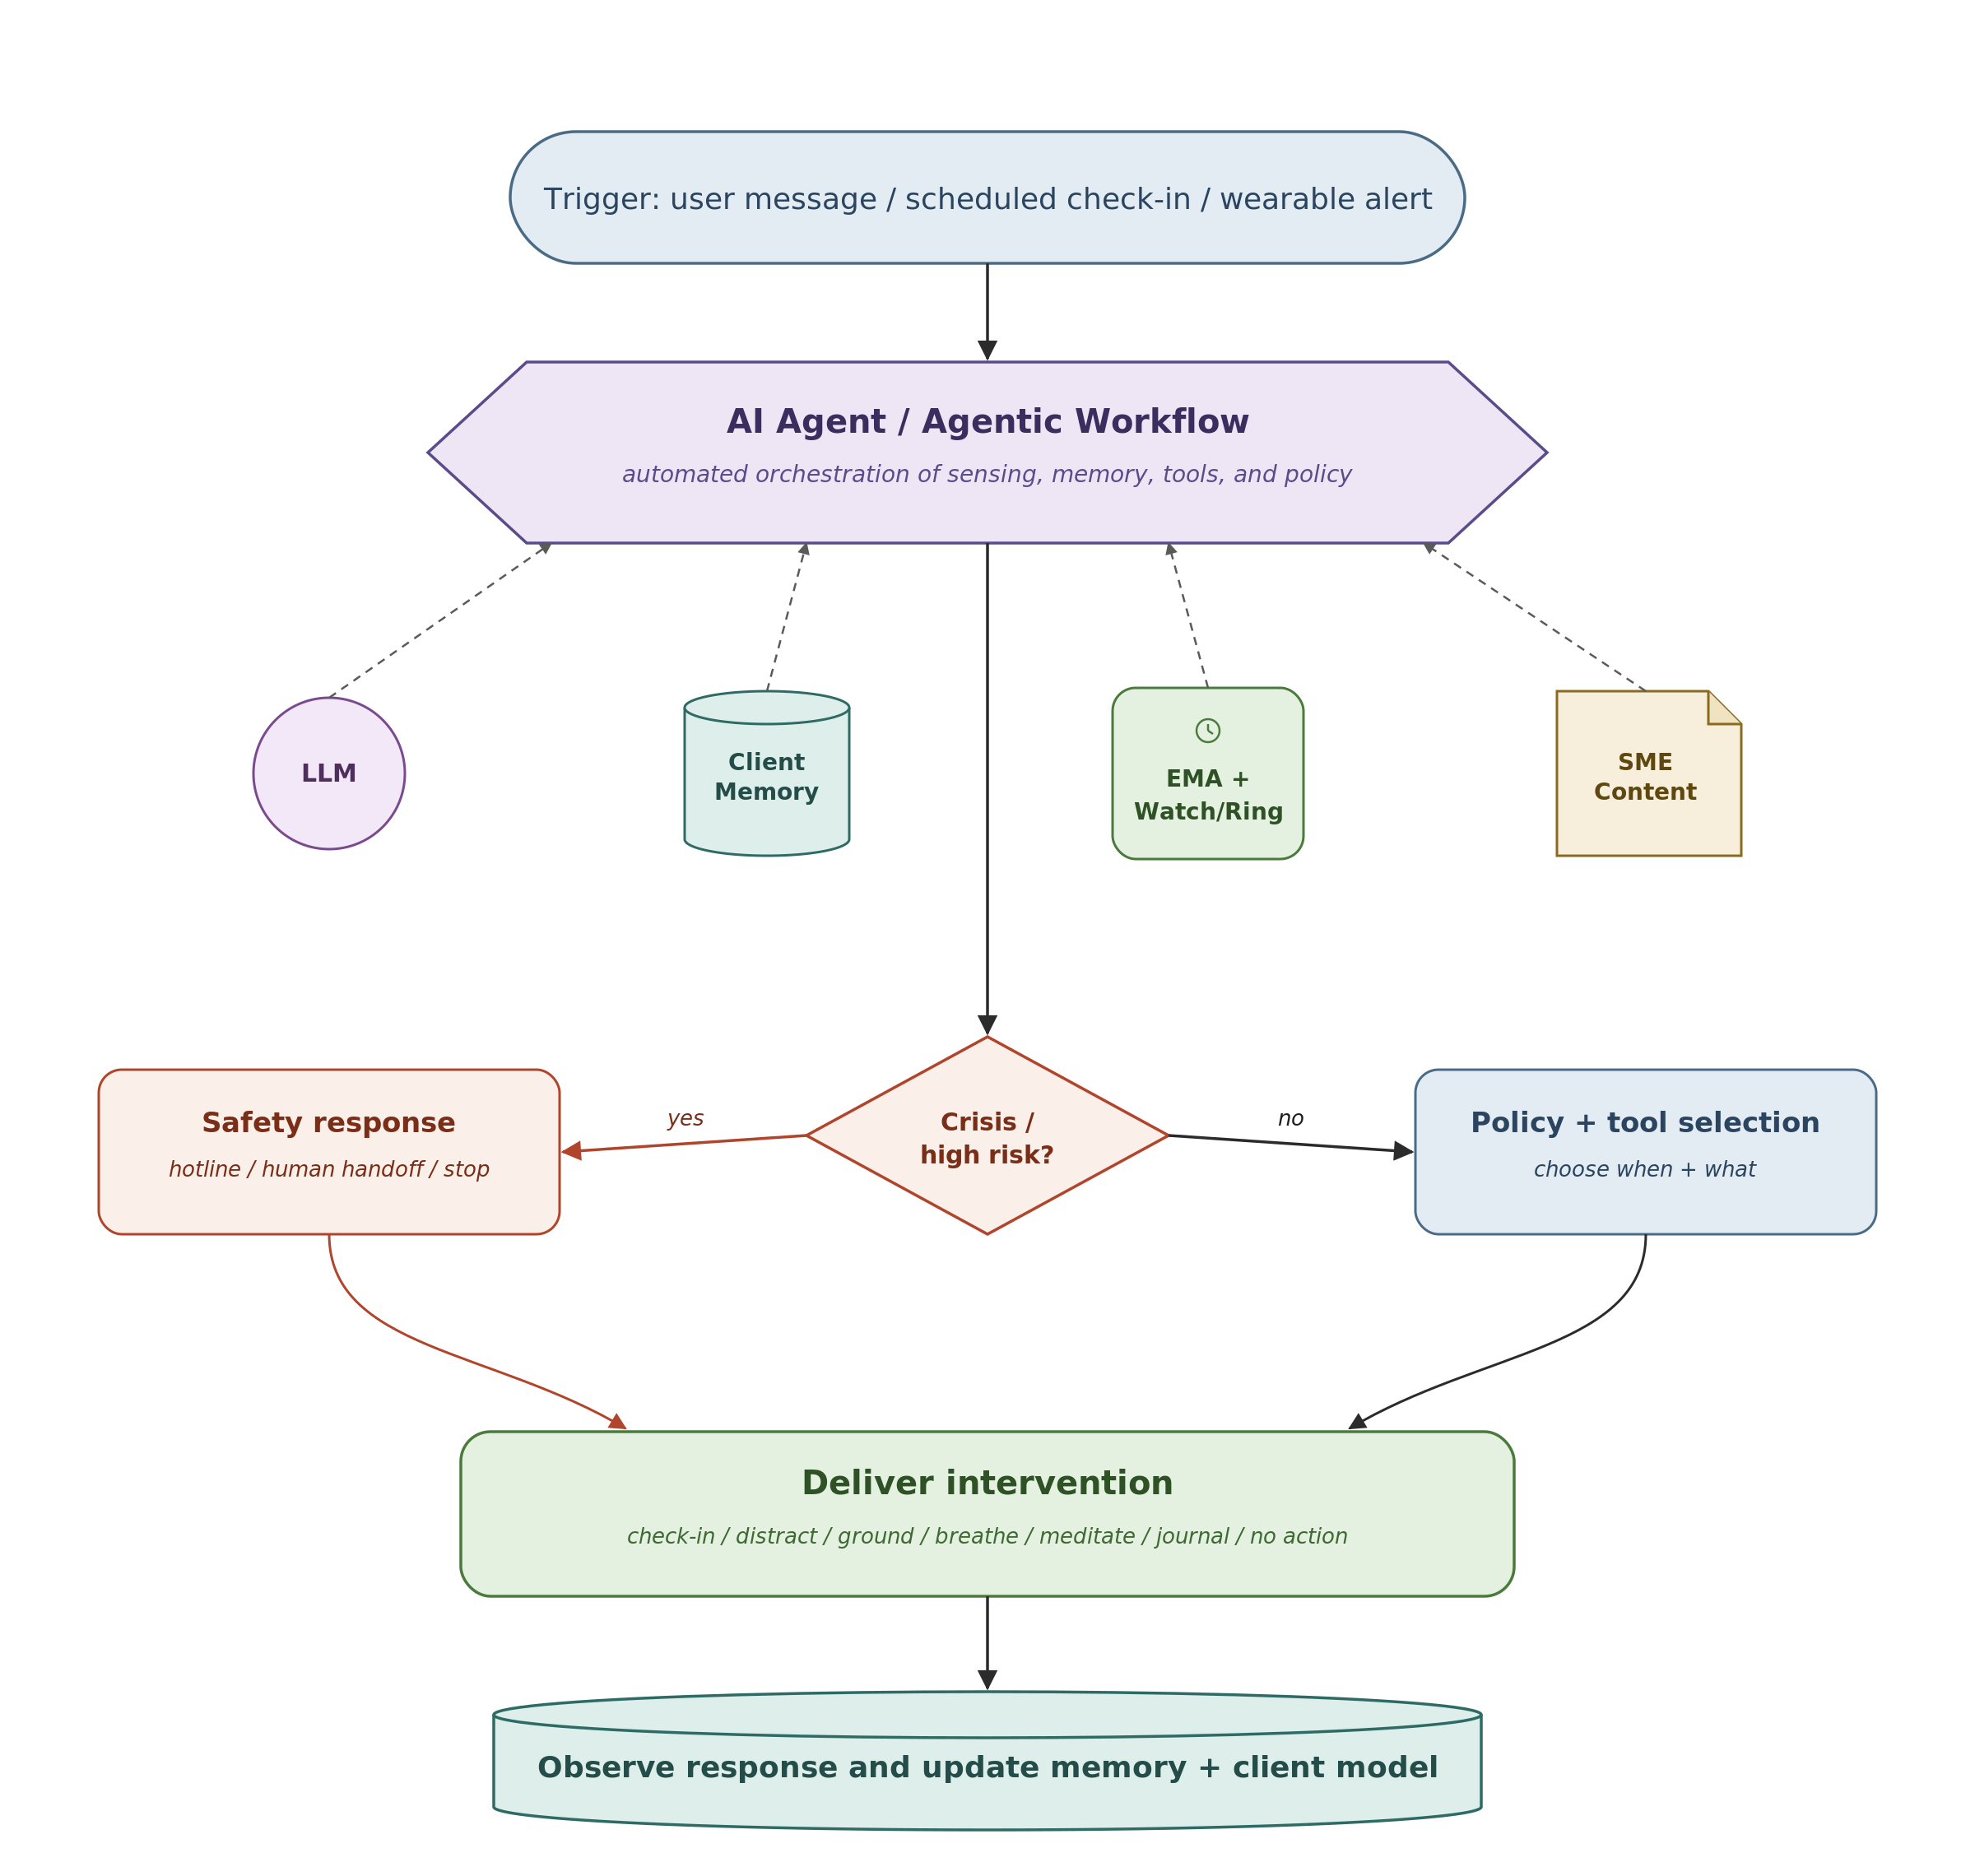
\includegraphics[width=1\linewidth]{figure1.png}
\caption{Architectural view of the proposed adaptive check-in
workflow. A trigger (user message, scheduled check-in, or
wearable alert) enters an orchestration node that combines an
LLM, client memory, EMA or wearable signals, and SME-authored
content; a risk gate branches to crisis handling when needed;
otherwise a Decide policy selects a low-risk intervention from the
SME-authored catalogue, the response is delivered through the
chat substrate, and the client-model state is updated for the
next loop. Wearable signals are a future, opt-in extension rather
than the baseline substrate.}
\label{fig:sda-loop}
\end{figure}

\subsection{Feasibility of a Candidate Integrated System}\label{sec:feasibility}

The question is whether every subsystem in a \mbox{C1--C5}-compliant
integrated system has a credible literature-backed implementation
path that avoids new model training. \tabref{tab:feasibility}
summarizes.

\begin{table}[t]
\small
\begin{tabularx}{\textwidth}{l X}
\toprule
\textbf{Subsystem} & \textbf{Existing evidence / primary risk} \\
\midrule
Sense & LLM-based state inference on chat data~\cite{Xu2024MentalLLM,Stade2024LLMOppRisks};
interpretable lexical features~\cite{Walker2024InstagramSuicideLIWC,Boettcher2021RedditMHReview};
optional EMA / wearable layer~\cite{Trull2009ESMEMA,Versluis2016EMI,Sequeira2021PassiveSensing,Laborde2017HRV}.
\emph{Risk:} hallucinated specificity in the language layer;
calibration failure at individual scale; false positives from
noisy wearable signals; ethical concerns about state-inference as
surveillance~\cite{BirkSamuel2020DigitalPhenotypingCritique}. \\
Decide & JITAI framework~\cite{NahumShani2018JITAI};
MRT~\cite{Klasnja2015MRT,Liao2016MRTSampleSize}; online
RL~\cite{Liao2020PersonalizedHeartSteps}; offline CMAB in emotion
regulation~\cite{Ameko2020CMABEmotion}; mental-health RCT
precedent~\cite{Aguilera2024DIAMANTERL}; behavior-change
taxonomies~\cite{Michie2011BCW,Michie2013BCTTaxonomy}.
\emph{Risk:} reward-specification error (optimizing engagement at
the expense of clinical value); policy instability at small N. \\
Act & Established by current LLM-chat deployment patterns that
assemble SME-authored method and safety constraints into the system
prompt; RCT precedent
across three agents~\cite{Fitzpatrick2017Woebot,Inkster2018Wysa,Heinz2025TherabotRCT};
meta-analytic support for CBT-based chat~\cite{Linardon2019Meta}.
\emph{Risk:} alliance drift~\cite{Henson2019DTA,MalouinLachance2025DTAReview};
process-vs-content confusion. \\
Crisis & Keyword detector; moderation API; LLM safety classifier;
validation against C-SSRS~\cite{Posner2011CSSRS}.
\emph{Risk:} false negatives (catastrophic); keyword list staleness. \\
Evaluation & MRT~\cite{Klasnja2015MRT,Liao2016MRTSampleSize,Luers2018StandardizedEffect,Seewald2019MRTData};
WAI-SR~\cite{Hatcher2006WAISR}; attrition-curve
benchmark~\cite{Linardon2020Attrition}.
\emph{Risk:} human evaluation cost; longitudinal follow-up
attrition; small N. \\
Ethics / governance & WHO-aligned ethical
principles~\cite{MartinezMartin2021DigitalPhenotypingEthics,MartinezMartin2020COVIDDigitalMHEthics};
transparent consent; SME-owned content; documented governance
architecture~\cite{vanHeerden2023LLMGlobalMH}. \emph{Risk:}
regulatory drift between US Food and Drug Administration ``wellness
app'' and ``software as a medical device'' (SaMD) classifications
as capability grows. \\
\bottomrule
\end{tabularx}
\caption{Feasibility assessment of a candidate integrated system
satisfying criteria~C1--C5.}
\label{tab:feasibility}
\end{table}

The synthesis supports a guarded but actionable conclusion: based
on the literature reviewed here, no subsystem appears to require
training a new foundation model. The remaining work is primarily
an integration problem coupled to a human-subjects evaluation,
subject to the residual risks per row of \tabref{tab:feasibility}
(reward-specification error in the Decide layer; calibration
failure of LLM-based state inference at individual scale;
catastrophic false negatives in the crisis layer; alliance drift
in the Act layer; regulatory drift between US Food and Drug
Administration ``wellness app'' and SaMD classifications as
capability grows). Within those constraints, the review supports a
specific implementation order: a \emph{Decide-first} prototype,
because the policy layer is the narrowest subsystem with the
strongest low-cost evaluation design (the MRT), and because the
Sense substrate for a chat-only deployment is already available
via the same LLM that powers \emph{Act}.

% =============================================================================
\section{Discussion}\label{sec:discussion}

\subsection{Principal Results}\label{sec:principal-results}

This scoping review establishes three principal results.
\emph{First}, no peer-reviewed system within the surveyed corpus
jointly satisfies the five operational criteria \mbox{C1--C5} of an
integrated, learned, theory-grounded, scheduled check-in workflow
for a conversational mental health companion (\secref{sec:gap}).
\emph{Second}, the empirical literature supports the design choices
such a system would commit to: a longitudinal chat-derived client
model~\cite{Xu2024MentalLLM,Wang2020COVIDStudentLife}, a JITAI-style
scheduling policy with MRT
evaluation~\cite{NahumShani2018JITAI,Klasnja2015MRT}, conversational
delivery with explicit crisis-safe
fallbacks~\cite{Heinz2025TherabotRCT,DeFreitas2024ChatbotSafety},
and engagement-aware reporting alongside proximal
effects~\cite{Linardon2020Attrition}. \emph{Third}, every technical
component required to fill the gap is already available through
currently accessible models, established software patterns, or open
methodology, making the integration tractable without any new
foundation-model
training~(\tabref{tab:feasibility}).

\subsection{Comparison With Prior Work}\label{sec:comparison}

This review extends three prior bodies of work in distinct ways.

The recent qualitative systematic review of Nahum-Shani et
al.~\cite{NahumShani2025JITAIMHReview} documents that JITAI
deployment for clinical mental-health outcomes remains structurally
thin despite the methodological maturity of the JITAI/MRT/RL
stack. We extend that finding by demonstrating that the gap is
not for lack of available components: the Decide-pillar synthesis
in \secref{sec:decide} and the feasibility analysis of
\secref{sec:feasibility} together show that the
JITAI-on-conversational-substrate integration is constrained by
\emph{integration effort and trial commitment}, not by a missing
algorithm or unavailable measurement instrument.

The Linardon et al.~\cite{Linardon2019Meta} meta-analysis of 66
smartphone-intervention RCTs establishes that engagement reminders
and professional guidance are the strongest moderators of effect
size in app-supported mental health interventions. We reframe
this finding from the Decide-pillar perspective: ``engagement
reminders'' is a degenerate special case of the much richer
adaptive-scheduling policy class developed in mHealth
biostatistics, and the meta-analytic evidence accordingly
establishes a \emph{lower bound} on what scheduling intelligence
can contribute, not a ceiling.

The Malouin-Lachance et al.~\cite{MalouinLachance2025DTAReview}
DTA review proposes goal/task/bond/engagement as the four working
elements of digital therapeutic alliance. We connect this
construct directly to the action space of an integrated companion:
the same four elements the alliance literature foregrounds are the
four elements a Decide policy must operate over (what goal to
pursue, what task to offer, how warmly to speak, when to prompt).
This connection has not, to our knowledge, been made explicit in
the published literature on either DTA or JITAIs.

Finally, no prior work that we identified frames the integration
problem as an explicit \mbox{C1--C5} criterion set. The criterion
set is itself a contribution: it provides a vocabulary in which
existing systems can be located on the design space, future
systems can be benchmarked, and reviewers can identify what is
missing in any given submission.

\subsection{Limitations}\label{sec:limitations}

As a scoping review with a feasibility framing, this paper has
five explicit limitations.

(i)~\emph{Single-reviewer screening.} A single reviewer screened
every record returned by the twelve Boolean queries; PRISMA-2020
and PRISMA-ScR both recommend double-screening, and a future
revision should add an independent screener and report
inter-rater agreement~\cite{Tricco2018PRISMAScR,Page2021PRISMA}.

(ii)~\emph{No formal risk-of-bias scoring.} The review synthesizes
evidence narratively across HCI, mHealth biostatistics, clinical
psychology, behavior-change science, and natural language
processing; we did not apply a quantitative risk-of-bias
instrument because no single instrument is appropriate across
these heterogeneous evaluation designs.

(iii)~\emph{Industry sources as dated snapshots.} Documented
chatbot-harm cases (Replika, NEDA Tessa, Character.AI) are
surfaced by~\cite{DeFreitas2024ChatbotSafety} and~\cite{Scholich2025TherapistVsChatbot}
rather than being cited as primary industry sources; we have not
independently verified press reports and do not treat them as
load-bearing.

(iv)~\emph{Scope.} The review covers English-language, adult,
text-chat-modality digital mental health. Multilingual deployment,
adolescent and older-adult populations, voice/video modalities, and
clinical-grade care (therapist replacement vs.\ augmentation) are
each their own review; they are flagged as priorities for future
revisions.

(v)~\emph{Ethical asymmetry of the framing.} Treating
mental-state changes as a \emph{policy-optimization problem}
(\secref{sec:decide}) imports the reward-specification problem
from RL into a domain where the reward is not clinically
uncontroversial. We discuss this in \secref{sec:ethics-results}; a
future revision should engage the clinical-ethics literature more
fully than a scoping-review format allows.

\subsection{Conclusions}\label{sec:conclusions}

\paragraph{Status of the present work.}
This paper is a literature review and a research agenda. It does
not report a built prototype, a user study, or any clinical or
behavioral outcomes. As an illustrative exemplar of the
architectural class proposed in
\secref{sec:gap}--\ref{sec:feasibility}, we point to one candidate
implementation under private development by the author (hereafter,
Willow) which currently
realizes only the conversational delivery layer (C3 $+$ C4) plus
a Phase-0 keyword crisis stack; the \emph{Sense} layer (C1), the
\emph{Decide} scheduling policy (C2), and any prospective
evaluation that this review motivates have not yet been
implemented. Willow is referenced here as one possible carrier of
the research agenda, not as the unit of evaluation; an SME team
adopting a different chat substrate, framework, or hosting model
could equally instantiate the C1--C5 architecture.

\paragraph{Proposed research agenda.}
The recommended next step is a \emph{Decide-first prototype}
followed by a micro-randomized trial:

\begin{itemize}\setlength{\itemsep}{0pt}
  \item \textbf{Stage 1 (this paper).} Lit-review-driven scoping
    and research agenda. Establish C1--C5, the comparison
    shortlist, and the feasibility map. \emph{Status: this paper.}
  \item \textbf{Stage 2 (next).} Implement the Decide layer: a
    small Thompson-sampling contextual-bandit scheduler over an
    existing chat substrate (e.g., the candidate exemplar named
    above) that selects (a)~when to proactively reach out and
    (b)~which technique to offer from a BCT-aligned, SME-authored
    intervention catalogue.
  \item \textbf{Stage 2b (optional sensing extension).} Add an
    explicit-consent wearable branch to the Sense layer, using
    watch or ring signals (e.g., sleep, activity, HRV,
    temperature, recovery proxies) as timing cues for low-risk
    interventions such as distraction, grounding, breathing, or
    meditation prompts.
  \item \textbf{Stage 3.} A micro-randomized
    trial~\cite{Klasnja2015MRT,Liao2016MRTSampleSize,Seewald2019MRTData}
    at $N\!\approx\!30\text{--}50$ participants benchmarked
    against the comparison shortlist of \tabref{tab:comparison},
    with the three-way reporting matrix of
    \secref{sec:evaluation} (MRT proximal effects; WAI-SR
    alliance; retention curves).
  \item \textbf{Stage 4.} A larger preregistered RCT, comparable
    in design to~\cite{Aguilera2024DIAMANTERL} and the
    \textit{NEJM~AI} Therabot trial of~\cite{Heinz2025TherabotRCT}.
\end{itemize}

More generally, we argue that this problem belongs at the
intersection of digital-mental-health biostatistics, HCI, clinical
psychology, and AI safety, and that an explicit
SME$\,\leftrightarrow\,$developer content-separation architecture
is a defensible substrate for a research agenda that takes all
four of those disciplines seriously. The present paper contributes
the review and the agenda; the prototype, the MRT, and the RCT are
sequential next steps.

% =============================================================================
% Front-matter end-sections required by JMIR Mental Health
% =============================================================================

\section*{Acknowledgments}\label{sec:ack}
The author thanks the SME and developer collaborators on the
Willow research project for early feedback on which sections of
the literature warranted the deepest synthesis, and the
\emph{JMIR Mental Health} editorial team for the venue's
sustained attention to digital-mental-health methodology.

\section*{Funding Statement}\label{sec:funding}
This work received no specific grant funding. The candidate
implementation referenced in the manuscript (Willow) is maintained
without external funding by the author.

\section*{Conflicts of Interest}\label{sec:coi}
The author declares no commercial conflicts of interest. The
author is the developer of Willow, a privately maintained research
software system referenced in the manuscript as an illustrative
candidate implementation. Willow is not publicly released and does
not generate revenue or investment. No author or affiliated institution holds equity in,
or receives consulting income from, any of the chatbot or
mHealth platforms cited in this manuscript.

\section*{Data Availability}\label{sec:data-availability}
This is a literature review. No new human-subject data were
generated or analyzed. The PRISMA-ScR checklist and full search
strategy are included as Multimedia Appendices~1 and~2. Internal
code, development materials, and any non-public data assets
associated with the candidate implementation discussed in the
manuscript are outside the scope of this review and are not
publicly shared.

\section*{Authors' Contributions}\label{sec:contributions}
M.M.\ is the sole author and was responsible for conceptualization,
search strategy design, screening, data charting, narrative
synthesis, drafting, and revision of the manuscript. M.M.\ approved
the final version for submission and assumes full responsibility
for the scientific content and reference validity of this paper.

\section*{Abbreviations}\label{sec:abbrev}
\begin{description}\setlength{\itemsep}{0pt}
  \item[ACT] acceptance and commitment therapy
  \item[AI] artificial intelligence
  \item[BCT] behavior change technique
  \item[BCW] Behaviour Change Wheel
  \item[CBT] cognitive behavioral therapy
  \item[CFT] compassion-focused therapy
  \item[CMAB] contextual multi-armed bandit
  \item[COM-B] capability--opportunity--motivation $\to$ behavior
  \item[C-SSRS] Columbia-Suicide Severity Rating Scale
  \item[DBT] dialectical behavior therapy
  \item[DOI] digital object identifier
  \item[DTA] digital therapeutic alliance
  \item[EMA] ecological momentary assessment
  \item[EMI] ecological momentary intervention
  \item[GAD] generalized anxiety disorder
  \item[GAD-7] Generalized Anxiety Disorder 7-item scale
  \item[HCI] human--computer interaction
  \item[HRV] heart-rate variability
  \item[IRB] Institutional Review Board
  \item[JITAI] just-in-time adaptive intervention
  \item[LIWC] Linguistic Inquiry and Word Count
  \item[LLM] large language model
  \item[MDD] major depressive disorder
  \item[mHealth] mobile health
  \item[MI] motivational interviewing
  \item[MRT] micro-randomized trial
  \item[MSC] Mindful Self-Compassion
  \item[NLP] natural language processing
  \item[PHQ-9] Patient Health Questionnaire 9-item
  \item[PRISMA] Preferred Reporting Items for Systematic Reviews and Meta-Analyses
  \item[PRISMA-ScR] PRISMA Extension for Scoping Reviews
  \item[PTSD] post-traumatic stress disorder
  \item[RCT] randomized controlled trial
  \item[RL] reinforcement learning
  \item[SaMD] software as a medical device
  \item[SFBT] solution-focused brief therapy
  \item[SME] subject matter expert
  \item[WAI-SR] Working Alliance Inventory-Short Revised
  \item[WHO] World Health Organization
\end{description}

\section*{Multimedia Appendices}\label{sec:multimedia}
\begin{description}\setlength{\itemsep}{0pt}
  \item[\textbf{Multimedia Appendix 1.}] PRISMA-ScR (Preferred Reporting
    Items for Systematic Reviews and Meta-Analyses Extension for
    Scoping Reviews) checklist for this review. File:
    \texttt{appendix-1-prisma-scr-checklist.md}.
  \item[\textbf{Multimedia Appendix 2.}] Full search strategy
    specification: per-query Boolean search terms, fields searched,
    date range, retrieval service, parameter values, and
    post-screening retention. File:
    \texttt{appendix-2-search-strategy.md}.
\end{description}

% =============================================================================
% Optional but recommended JMIR sections
% =============================================================================

\section*{AI Usage Statement}\label{sec:ai-usage}
We disclose the following uses of AI tools in the preparation of
this manuscript.
(i)~\textit{Verified literature search.} The Scite MCP
(\url{https://api.scite.ai}) was used to retrieve DOI metadata,
full-text excerpts, smart citation context (supporting /
contrasting / mentioning / unclassified), and editorial-notice
flags for every cited source. Every citation in this paper has a
DOI independently verified against Scite's index; no citation was
generated, invented, or paraphrased from an LLM's parametric
memory.
(ii)~\textit{Drafting and synthesis assistance.} An LLM-based
coding assistant (Claude) operating inside the Cursor IDE was used
to assist with prose drafting, reorganization, and synthesis
across sections of this review. All research questions,
inclusion/exclusion decisions, the taxonomy, claims, comparative
analyses, feasibility judgments, and conclusions were authored and
verified by the human author, who assumes full responsibility for
the scientific content and reference validity of this paper.
(iii)~\textit{Editing.} Standard grammar correction and clarity
editing tools were used in a copy-editing role.
The review reports no new experimental results; no AI tool was
used to generate or alter experimental data, analyses, or figures.

\section*{Ethics Statement}\label{sec:ethics-statement}
This is a literature review and contains no new human-subjects
data; IRB approval was not required for this work, and no
participants were recruited. The review nonetheless touches four
ethics-relevant areas that any future system building on this
synthesis must address.

(i)~\emph{Mental-state inference as a surveillance risk.} Any
system that implements Pillar~A (Sense) learns an inferred state
representation of the user; the sociological critique
of~\cite{BirkSamuel2020DigitalPhenotypingCritique} and the
ethical-governance recommendations
of~\cite{MartinezMartin2021DigitalPhenotypingEthics} together set
the minimum bar: the representation must be inspectable by the
user, resettable on request, and never shared or sold.

(ii)~\emph{Engagement-optimization as a misaligned reward.} The
Decide pillar treats intervention scheduling as a
policy-optimization problem (\secref{sec:decide}). The reward
function matters more than the algorithm. A policy that silently
optimized for engagement at the cost of clinical value would be
strictly worse than a fixed schedule; any future
prototype---Willow included---must explicitly separate
\emph{engagement proxies} from \emph{therapeutic-goal proxies} in
the reward, and report both.

(iii)~\emph{Crisis-handoff responsibility.} The candidate
implementation (Willow) is explicitly \emph{not} a therapist,
doctor, or crisis service; the crisis layer exists to route users
to human help, not to substitute for it. The empirical
literature~\cite{DeFreitas2024ChatbotSafety,Scholich2025TherapistVsChatbot}
shows that general-purpose chat substrates are not safe defaults
for crisis, which is why the keyword detector (Phase~0) and any
downstream LLM-safety classifier (Phase~4) must be held to a
different evaluation standard than the rest of the action
catalogue: missed signals are not acceptable failure modes.

(iv)~\emph{Scope and equity.} The review's restriction to
English-language, adult, text-chat-modality interventions is a
scope limitation, not a normative claim. The global-equity framing
of~\cite{vanHeerden2023LLMGlobalMH} and the pandemic-era digital
access shifts of~\cite{MartinezMartin2020COVIDDigitalMHEthics}
both argue that access is itself a therapeutic outcome; an
evaluation of the proposed prototype must stratify on digital
literacy and language to avoid widening the very gap it aims to
close.

\printbibliography[heading=bibnumbered,title={References}]

\end{document}
